\documentclass[]{report}

\usepackage{import}

\import{../}{settings.tex}

\title{Analyse et Equations différentielles partielles}

\author{Cours de Xavier Blanc, transcrit par SADR TAHOURI Luca}
\date{}

\begin{document}

    \maketitle
    \tableofcontents

    \chapter{Préliminaires: Formules de Green, transformée de Fourier}

    \begin{nt}{}{}
        $\Omega$ ouvert connexe de $\R^d$ (souvent borné), $d\in \N^*$ et pour $k\in \N$
        \[k\in \N, C^k(\Omega)=\{\funto{f}{\Omega}{\R},f\text{ est de classe } C^k\}\]
        \[C^k_c(\Omega)=\{f\in C^k(\Omega), \text{supp}(f)\text{ compact de }\Omega\}\]
        \[C^k(\overline{\Omega})=\{f_{|\overline{\Omega}},f\in C^k(\R^d)\}\]
        Notations similaires si $f$ est à valeurs dans $\R^m$
    \end{nt}

    \section{Dérivées partielles}

    $f\in C^1(\Omega),x\in \Omega,x=(x_1,\ldots,x_d)$. On note $\frac{\partial f}{\partial x_i}(x)=\partial_i f(x)$ la dérivée partielle par rapport à $x_i$.\\
    Pour les dérivées d'ordre supérieur: $\alpha\in \N^d$ multi-indice, $\alpha=(\alpha_1,\ldots,\alpha_d),\alpha_i\in \N$.\\
    $\partial^\alpha f(x)=\partial_1^{\alpha_1}\ldots \partial_d^{\alpha_d} f$ et on note $|\alpha|=\sum_{i=1}^{d}\alpha_i\in \N$ longueur du multi-indice.Il faut avoir $f\in C^{|\alpha|}(\Omega)$
    
    \begin{ex}{}{}
        $d=3$, $\alpha=(1,0,2)$ et $\partial^\alpha f=\partial_1\partial_3^2 f=\frac{\partial^3f}{\partial x_1\partial x_2^2}$
    \end{ex}

    \begin{df}{}{}
        Soit $f\in C^1(\Omega)$, on appelle gradient de $f$ l'application:
        \[\fundfto{\nabla f}{\Omega}{\R^d}{x}{\left(\begin{matrix} \partial_1 f(x)\\ \vdots \\ \partial_d f(x) \end{matrix}\right)}\]
        On appelle divergence de $f$ l'application:
        \[\fundfto{\text{div} f}{\Omega}{\R}{x}{\sum_{i=1}^d\partial_i f(x)}\]
        Pour $f\in C^2(\Omega)$, on appelle lapplacien de f l'application:
        \[\fundfto{\Delta f}{\Omega}{\R}{x}{\sum_{i=1}^{d}\partial_i^2 f}\]
    \end{df}

    \begin{ex}{}{}
        $f(x_1,x_2,x_3)=x_1x_2^2e^{x_3}$
        \[\nabla f(x)=\left(\begin{matrix}
            x_2^2 e^{x_3}\\
            2x_1x_2 e^{x_3}\\
            x_1 x_2^2 e^{x_3}
        \end{matrix}\right)=\left( \begin{matrix}
            x_2\\
            2x_1\\
            x_1x_2
        \end{matrix}\right) x_2 e^{x_3}\]
    \end{ex}

    \begin{df}{}{}
        Soit $V\in C^1(\Omega,\R^d)$. On appelle divergence de $V$ l'application $\fundfto{\text{div} (V)}{\Omega}{\R}{x}{\sum_{i=1}^{d}\partial_i V_i(x)}$.\\
        Quelquefois noté $\nabla\cdot V$
    \end{df}

    \begin{ex}{}{}
        \[V(x)=\left(\begin{matrix}
            x_1\\
            x_3\\
            x_2^2 e^{x_1}
        \end{matrix}\right)\]
        \[\text{div}(V)=1+0+0=1\]
    \end{ex}

    \section{Formules de Green}

    Intégration par parties (en dimension $d$)

    \begin{ra}{}{}
        $d=1$, $\funto{f,g}{[a,b]}{\R}\in C^1$, alors
        \[\int_{a}^{b}f'g=\left[fg\right]_a^b-\int_{a}^{b} fg'\]
        En particulier, si $f,g\in C^1_C(]a,b[)$, $\int_{a}^{b} f'g=-\int_{a}^{b}fg'$
    \end{ra}

    \begin{prop}{}{}
        Soit $(f,g)\in C^1(\Omega)^2$, telles que $f$ ou $g$ soit à support compact, alors
        \[\int_{\Omega}\partial_i fg=-\int_{\Omega} f\partial_i g,\forall i\in \{1,\ldots,d\}\]
    \end{prop}

    \begin{ra}{Lemme d'Urysohn}{}
        Soit $X$ un espace normé. Soient $E,F$ parties fermées disjointes de $X$. Alors $\exists \Xr\in C^1(X)$ telle que $\Xr_{|F}=1$ et $\Xr_{|E}=0$ et $0\le \Xr\le 1$
    \end{ra}

    \begin{proof}
        On suppose $f$ à support compact dans $\Omega$. $F=\text{supp}(f)\subset \Omega, E=\Omega^C$, et $E,F$ sont fermés de $\R^d$.\\
        Par le lemme précédent, $\Xr\in C^1(\R^d),\Xr_{|F}=1,\Xr_{\Omega^C}=0, 0\le \Xr\le 1$.
        \[\int_\Omega \partial_i fg=\int_F \partial_i fg=\int_F \Xr \partial_i f g\]
        On pose $\tilde{g}(x)=\cho{\Xr(x)g(x)\text{ si $x\in \Omega$}\\0\text{ si $x\in \Omega^C$}}$. $\tilde{g}\in C^1(\R^d)$
        De même, $\tilde{f}(x)=\cho{f(x)\text{ si $x\in \Omega$}\\ 0\text{ si $x\in \Omega^C$}}$ et $\tilde{f}\in C^1$. On a alors
        \begin{align*}
            \int_\Omega \partial_i fg&=\int_F \partial_i \tilde{f}\tilde{g}=\int_{[-A,A]^d}\text{ où $A$ est tel que $F\subset [-A,A]^d$}\\
            &=\int_{-A}^{A}\ldots\int_{-A}^{A}\partial_i \tilde{f}(x)\tilde{g}(x)\, dx_1\ldots dx_d\\
        \end{align*}
        \[\int_{-A}^{A} \partial_i \tilde{f}(x)\tilde{g}(x)\, dx_i=\underset{=0}{\left[\tilde{f}\tilde{g}\right]_{x_i=-A}^{x_i=A}}-\int_{-A}^{A}\tilde{f}(x)\partial_i \tilde{g}(x)\, dx_i\]
        Donc $\int_\Omega \partial_i df=-\int_{[-A,A]^d}\tilde{f}\partial_i \tilde{g}$
        \[\int_\Omega \partial_i fg=-\int_F \tilde{f}\partial_i \tilde{g}=-\int_F f\partial_i g\]
    \end{proof}

    \begin{cor}{}{}
        Soit $f\in C^1(\Omega)$ et soit $V\in C^1(\Omega,\R^d)$, telles que $f$ ou $V$ soit à support compact, alors $\int_\Omega \nabla f\cdot V=-\int_\Omega f\text{div}(V)$
    \end{cor}

    \begin{proof}
        On applique la propriété précédente à $f$ et $g=V_i\in C^1(\Omega)$
        \[\int_\Omega \partial_i f V_i=-\int_\Omega f\partial_i V_i\]
        On somme sur $i$, $\sum_{i=1}^{d}\partial_i f V_i=\nabla f\cdot V$ et $\sum_{i=1}^{d}\partial_i V_i=\text{div}(V)$, d'où
        \[\int_\Omega \nabla f\cdot V=-\int_\Omega f\text{div}(V)\]
    \end{proof}

    \begin{re}{}{}
        Si $V=\nabla g,g\in C^2(\Omega)$, alors
        \[\int_\Omega \nabla f\cdot \nabla g=-\int_\Omega f\text{div}(\nabla g)=\int_\Omega f(-\Delta g)\]
        où $\Delta g$ est le laplacien de $g$, $\Delta g(x)=\sum_{i=1}^{d}\partial_i^2 g$
    \end{re}

    \begin{tm}{}{}
        Soit $\Omega$ un ouvert borné de $\R^d$, de classe $C^1$. Soit $(f,g)\in (C^1(\Omega)\cap C^0(\overline{\Omega}))^2$. Alors $\forall i\in \{1,\ldots,d\}$,
        \[\int_\Omega \partial_i fg=\int_{\partial \Omega}fg n_i\, d\sigma-\int_{\Omega}f\partial_i g\]
        où $n=n(x)$ normale sortante à $\Omega$ en $x\in \partial\Omega$, $n_i=n\cdot e_i=n\cdot\left(\begin{matrix}
            0\\
            \vdots\\
            0\\
            1\\
            0\\
            \vdots\\
            0
        \end{matrix}\right)$ et $\sigma$ est la mesure uniforme sur $\partial \Omega$
    \end{tm}

    \begin{df}{}{}
        $\Omega$ ouvert de $\R^d$ est dit de classe $C^1$ (à bord de classe $C^1$) s'il existe des ouverts $U_0,\ldots,U_n$ et $\varphi_0,\ldots,\varphi_n$ tels que
        \begin{itemize}
            \item $\overline{\Omega}\subset \bigcup_{i=0}^N U_i$
            \item $\overline{U_0}\subset \Omega$
            \item $\funto{\varphi_0}{U_0}{B_1(0)=\{x\in \R^d,|x|<1\}}$ est un $C^1$-difféomorphisme
            \item $\funto{\varphi_i}{U_i}{B_1(0)}$ sont des $C_1$-difféomorphismes et tels que $\varphi_i(U_i\cap \Omega)=\{x\in B_1(0),x_d>0\}$ et $\varphi_i(U_i\cap \partial \Omega)=\{x\in B_1(0),x_d=0\}$
        \end{itemize}

    \begin{tikzpicture}[>=Stealth,scale=1.1]

        % Omega
        \draw[thick] (0,0) ellipse (3 and 2);
        \node at (0,-2.2) {$\Omega$};

        % U0
        \draw[thick] (0,0) ellipse (2.7 and 1.9);
        \node at (0,-1.5) {$U_0$};

        % U2
        \draw[thick] (-2,1) ellipse (0.9 and 0.6);
        \node at (-2,1) {$U_2$};

        % U1
        \draw[thick] (-2.4,0.6) ellipse (0.8 and 0.7);
        \node at (-2.4,0.6) {$U_1$};

        % Ellipse à droite dans U0
        \draw[thick] (2.7,0) ellipse (0.9 and 1.2);

        % Partie hachurée
        \begin{scope}
            \clip (0,0) ellipse (2.7 and 1.9);
            \clip (2.7,0) ellipse (0.9 and 1.2);
            \fill[pattern=north east lines] (1.6,-1.5) rectangle (2.8,1.5);
        \end{scope}

        % Flèche vers la boule
        \draw[->,thick] (3.2,0.8) -- (6,0.8);
        \node at (4.6,1.1) {$\varphi_i$};

        % Flèche retour
        \draw[<-,thick] (3.2,-0.8) -- (6,-0.8);
        \node at (4.6,-1.1) {$\varphi_i^{-1}$};

        % Boule Bi(0)
        \draw[thick] (7.5,0) circle (1.3);
        \node at (8.3,1.2) {$B_i(0)$};

        % Demi-boule hachurée
        \begin{scope}
            \clip (7.5,0) circle (1.3);
            \fill[pattern=north east lines] (6.2,0) rectangle (8.8,1.5);
        \end{scope}

        % Ligne horizontale dans la boule
        \draw (6.2,0) -- (8.8,0);

        \end{tikzpicture}\\
        $d\sigma$ la mesure image de la mesure de Lebesque sur $B_1(0)\cap\{x_d=0\}$ par $\varphi_i$
    \end{df}

    \begin{re}{}{}
        $d\sigma$ ainsi défini ne dépend pas des $\Omega_i$ ni des $\varphi_i$. cf. JM Bony, Cours d'analyse, éditions de l'X
    \end{re}

    \begin{cor}{}{}
        Soit $\Omega$ ouvert borné de classe $C^1$, $f\in C^1(\Omega)\cap C^0(\overline{\Omega})$.\\
        $V\in C^1(\Omega,\R^d)\cap C^0(\overline{\Omega},\R^d)$ alors $\int_\Omega \nabla f\cdot V=\int_{\partial \Omega}f V\cdot n d\sigma- \int_\Omega f\text{div} (V)$
    \end{cor}

    \section{Transformée de Fourier}

    \begin{df}{}{}
        $\forall f\in L^1(\R^d)$, on définit $\widehat{f}(\zeta)=\int_{\R^d}f(x) e^{-2i\pi\zeta x}\, dx$ la transformée de Fourier de $f$, notée aussi $\Fr(f)=\widehat{f}$
    \end{df}

    \begin{prop}{}{}
        $\funto{\Fr}{L^1(\R^d)}{L^\infty(\R^d)}$ est linéaire continue
    \end{prop}

    \begin{proof}
        $\Fr$ est linéaire car l'intégrale est une forme linéaire.
        \begin{align*}
            \left\|\widehat{f}(\zeta)\right\|&\le \int_{\R^d}\left\|f(x)e^{-2i\pi x\zeta}\right\|\, dx\\
            &\le \int_{\R^d}\left\|f(x)\right\|\, dx=\norme{f}_{L^1(\R^d)}
        \end{align*}
        Donc $\widehat{f}\in L^\infty(\R^d)$ et $\norme{\widehat{f}}_{L^\infty(\R^d)}\le \norme{f}_{L^1(\R^d)}$
    \end{proof}

    \begin{re}{}{}
        \[\widehat{f}(0)=\int_{\R^d}f\]
    \end{re}

    \begin{ex}{}{}
        $d=1$, $f(x)=\1_{[-a,a]}(x)$
        \begin{align*}
            \widehat{f}(\zeta)&=\int_{\R}f(x)e^{-2i\pi x\zeta}\, dx\\
            &=\int_{-a}^{a}e^{-2i\pi \zeta}\, dx\\
            &=\frac{\sin (2\pi a \zeta)}{\pi \zeta}
        \end{align*}
    \end{ex}

    \begin{nt}{}{}
        $(f\in L_{\text{loc}}^1(\R^d))$
        \begin{itemize}
            \item $\forall h\in \R^d$, $\tau_h(f(x))=f(x-h)$
            \item $\Par f(x)=f(-x)$
            \item $\forall \zeta\in \R^d,e(\zeta)=e^{-2i\pi x\zeta}$
            \item $\forall \lambda\in\R^{+*},D_\lambda f(x)=f(\lambda x)$
            \item $L_{\text{loc}}^1(\R^d)=\{f\text{ mesurable, telle que $\forall \Omega\subset \R^d$ ouvert borné, $\int_{\Omega} \left|f(x)\right|\,dx <+\infty$}\}$
        \end{itemize}
    \end{nt}

    \begin{ra}{}{}
        \begin{itemize}
            \item Produit de convolution:
            \[\forall f\in L^1(\R^d),\forall g\in L^1(\R^d),(f*g)(x)=\int_{\R^d}f(y)g(x-y)\, dy\]
            \item Inégalité de Young: $\forall f\in L^p(\R^d),\forall g\in L^q(\R^d),f*g\in L^r(\R^d)$, avec $\frac{1}{p}+\frac{1}{q}=1+\frac{1}{r}$ et
            \[\norme{f*g}_{L^r(\R^d)}\le \norme{f}_{L^p(\R^d)}\norme{g}_{L^q(\R^d)}\]
        \end{itemize}
    \end{ra}

    \begin{prop}{}{}
        $\forall f\in L^1(\R^d),\forall g\in L^1(\R^d)$,
        \begin{itemize}
            \item $\widehat{f*g}(\zeta)=\widehat{f}(\zeta)\widehat{g}(\zeta)$
            \item $\int_{\R^d}\widehat{f}g=\int_{\R^d}f\widehat{g}$
            \item $\forall h\in \R^d, \widehat{\tau_h f}=e_h\widehat{f}, \widehat{e_h f}=\tau_h \widehat{f}$
            \item $\forall \lambda >0, \widehat{D_\lambda f}=\lambda^{-d}D_{\lambda^{-1}}\widehat{f}$
        \end{itemize}
    \end{prop}

    \begin{proof}
        \begin{itemize}
            \item \begin{align*}
                \widehat{f*g}&=\int_{\R^d} e^{-2i\pi x\zeta}\left(\int_{\R^d} f(y)g(x-y)\, dy\right)\, dx\\
                &=\int_{\R^d}\int_{\R^d}f(y)e^{-2i\pi y\zeta}g(x-y)e^{-2i\pi(x-y)\zeta}\,dy\, dx\\
                &=\int_{\R^d}f(y)e^{-2i\pi y\zeta}\left(\int_{\R^d}g(x-y)e^{-2i\pi (x-y)\zeta}\, dx\right)\, dy\\
                &=\widehat{f}(\zeta)\widehat{g}(\zeta)
            \end{align*}
            \item \begin{align*}
                \int_{\R^d}\widehat{f}(\zeta)g(\zeta)d\zeta&=\int_{\R^d}\int_{\R^d} f(x) e^{-2i\pi x\zeta}g(\zeta)\, dx\, d\zeta\\
                &= \int_{\R^d} f(x)\left(\int_{\R^d} g(\zeta)e^{-2i\pi x\zeta}\, d\zeta\right)\, dx=\int_{\R^d}f(x)\widehat{g}(x)\, dx
            \end{align*}
            \item \begin{align*}
                \widehat{\tau_h f(\zeta)}&=\int_{\R^d} e^{-2i\pi x\zeta} f(x-h)\, dx\\
                &=\int_{\R^d} e^{-2i\pi (y+h)\zeta} f(y)\, dy\\
                &=e^{-2i\pi h \zeta}\int_{\R^d}e^{-2i\pi y\zeta}f(y)\, dy\\
                &=e_h(\zeta)\widehat{f}(\zeta)
            \end{align*}
            \begin{align*}
                \widehat{e_h f}(\zeta)&=\int_{\R^d}e^{-2i\pi x\zeta}e^{-2i\pi hx} f(x)\, dx\\
                &=\int_{\R^d} e^{-2i\pi(\zeta+h)x}f(x)\, dx\\
                &=\widehat{f}(\zeta+h)=(\tau_{-h}\widehat{f})(\zeta)
            \end{align*}
            \item $\lambda>0$,
            \begin{align*}
                \widehat{D_\lambda f}(\zeta)&=\int_{\R^d}e^{-2i\pi\zeta x}f(\lambda x)\, dx\\
                &=\int_{\R^d}e^{-2i\pi \zeta\frac{y}{\lambda}} f(y)\lambda^{-d}\, dy=\lambda^{-d} \widehat{f}\left( \frac{\zeta}{\lambda}\right)\\
                &=\left(\lambda^{-d}D_{\lambda^{-1}}\widehat{f}\right)(\zeta)
            \end{align*}
        \end{itemize}
    \end{proof}

    \begin{prop}{}{}
        \begin{itemize}
            \item Si $f\in L^1(\R^d)$ et $(x\mapsto \left|x\right|f(x))\in L^1(\R^d)$, alors $\widehat{f}$ est dérivable, et $\forall j\in \{1,\ldots,d\},\partial_{\zeta_j}\widehat{f}(\zeta)=-2i\pi  \widehat{ x_j f}(\zeta)$
            \item Si $f\in L^1(\R^d)\cap C^1(\R^d)$, avec $\nabla f\in L^1(\R^d)$, alors $\forall j\in \{1,\ldots,d\}$
            \[\widehat{\partial_{\zeta_j}}(\zeta)=2i\pi \zeta_j \widehat{f}(\zeta)\]
        \end{itemize}
    \end{prop}

    \begin{proof}
        \begin{itemize}
            \item $\widehat{f}(\zeta)=\int_{\R^d}\underset{F(x,\zeta)\in L^1(\R^d)\text{ en x}}{e^{-2i\pi\zeta x}f(x)}\, dx$ et $\partial_{\zeta_j}F(x,\zeta)=-2i\pi x_j e^{-2i\pi\zeta x}f(x)\in L^1(\R^d)$ en $x$, uniformément en $\zeta$.\\
            Donc, par le TCD ou dérivation sous le signe intégral, $\widehat{f}$ dérivable, et
            \[\partial_{\zeta_j}\widehat{f}(\zeta)=\int_{\R^d}-2i\pi x_j e^{-2i\pi \zeta x}f(x)\, dx=\widehat{-2i\pi x_j f}(\zeta)\]
            \item On suppose d'abord $f$ à support compact.
            \begin{align*}
                \widehat{\partial_{x_j}f}(\zeta)&=\int_{\R^d}e^{-2i\pi x\zeta}\partial_{x_j}f(x)\, dx\\
                &=-\int_{\R^d}\partial_{x_j}(e^{-2i\pi x\zeta})f(x)\, dx\\
                &=-\int_{\R^d}(-2i\pi\zeta_j)e^{-2i\pi x \zeta}f(x)\, dx=2i\pi \zeta_j \widehat{f}(\zeta)
            \end{align*}
        \end{itemize}
    \end{proof}

    Idée: $C_C^\infty(\R^d)$ est dense dans $L^1(\R^d)\cap C^1(\R^d)$:\\
    \[\Xr\in C_C^\infty(\R^d),\cho{\Xr_{|B_1}=1\\ \Xr(x)=0,\forall x\in B_2^C\\ 0\le \Xr\le 1}\]
    \begin{tikzpicture}
    \begin{axis}[
        axis lines=middle,
        xmin=-3, xmax=3,
        ymin=-0.2, ymax=1.3,
        xtick={-2,-1,1,2},
        ytick=\empty,
        width=12cm,
        height=6cm,
        samples=300,
        domain=-3:3
    ]

    % Fonction de transition lisse
    \addplot[thick] 
    {
        (x <= -2) * 0
        + (x > -2 && x < -1) *
        (exp(-1/((x+2))) /
        (exp(-1/((x+2))) + exp(-1/(1-(x+2)))))
        + (x >= -1 && x <= 1) * 1
        + (x > 1 && x < 2) *
        (exp(-1/((2-x))) /
        (exp(-1/((2-x))) + exp(-1/(1-(2-x)))))
        + (x >= 2) * 0
    };

    \end{axis}
    \end{tikzpicture}\\
    $\Xr_n(x)=\Xr\left(\frac{x}{n}\right)$,$f\Xr_n$ est à support compact, donc
    \[\widehat{\partial_{x_j}(f \Xr_n)}(\xi)=2i\pi \xi_j \widehat{\Xr_n f}(\xi)\]
    \[\widehat{\Xr_n f}(\xi)=\int_{\R^d}e^{-2i\pi x\cdot \xi}\underset{\toninfty f(x)\text{ p.p.}}{\Xr_n(x)f(x)}\, dx\text{ et }\left|e^{-2i\pi x\cdot \xi}\Xr_n(x)f(x)\right|\le |f(x)|,f\in L^1(\R^d)\]
    Par TCD: $\widehat{\Xr_n f}(\xi)\toninfty \widehat{f}(\xi)$
    \begin{align*}
        \partial x_j(f\Xr_n)&=\partial x_j f\Xr_n+f\partial x_j \Xr_n\\
        \widehat{\partial x_j(f\Xr_n)}=\underset{\toninfty \widehat{\partial x_j f}}{\widehat{\partial x_j f \Xr_n}}+\widehat{f \partial x_j \Xr_n}
    \end{align*}
    Il reste à prouver que $\widehat{f\partial x_j \Xr_n}\toninfty 0$
    \[\left|\widehat{f\partial x_j\Xr_n}\right|(\xi)\le \int_{\R^d}|f(x)|\partial x_j \Xr_n(x)|\, dx\qquad \partial x_j \Xr_n=\frac{1}{n}\partial x_j \Xr\left(\frac{x}{n}\right)\]

    \begin{prop}{Lemme de Riemann-Lebesgue}{}
        $\forall f\in L^1(\R^d), \lim_{|\zeta|\to \infty}\widehat{f}(\zeta)=0$
    \end{prop}

    \begin{re}{}{}
        On sait aussi que $\zeta\mapsto \widehat{f}(\zeta)$ est continue si $f\in L^1$(continuité des intégrales à paramètres)
    \end{re}

    \begin{proof}
        Dans le Rudin
    \end{proof}

    \begin{prop}{}{}
        Soit $f\in L^1(\R^d)$ telle que $\widehat{f}\in L^1(\R^d)$, alors
        \[f(x)=\int_{\R^d}e^{2i\pi\zeta x}\widehat{f}(\zeta)d\zeta\]
    \end{prop}

    \begin{re}{}{}
        Ceci équivaut à $\Par \Fr=\Fr^{-1}$
    \end{re}

    \begin{proof}
        On pose $F(x)=\int_{\R^d}e^{2i\pi x\zeta}\widehat{f}(\zeta)\, d\zeta$ (on veut prouver $F=f$)\\
        \begin{align*}
            F(x)&=\int_{\R^d}\int_{\R^d} e^{2i\pi x\zeta} e^{-2i\pi y\zeta}f(y)\, dy\, d\zeta
        \end{align*}
        On pose
        \begin{align*}
            F_\epsilon(x)&=\int_{\R^d}\int_{\R^d}e^{2i\pi(x-y)\zeta}e^{-\epsilon \sum_{i=1}^{d}|\zeta_i|}f(y)\, dy\, d\zeta\qquad \text{ Par le TCD: $F_\epsilon(x)\underset{\epsilon}{\longrightarrow}F(x)$}
            &=\int_{\R^d}\left(\int_{\R^d}e^{2i\pi(x-y)\zeta}e^{\epsilon\sum_{i=1}^{d}|\zeta_i|}\, d\zeta\right)f(y)\, dy \qquad\text{(Par Fubini)}
        \end{align*}
        \begin{align*}
            \int_{\R^d}e^{2i\pi(x-y)\zeta-\epsilon\sum_{j=1}^{d}|\zeta_j|}\, d\zeta&= \int_{\R^d}e^{\sum_{j=1}^{d}(2i\pi(x_j-y_j)\zeta_j-\epsilon |\zeta_j|)}\, d\zeta\\
            &=\int_{\R^d}\prod_{j=1}^{d}\left(e^{2i\pi(x_j-y_j)\zeta_j-\epsilon |\zeta_j|}\right)\, d\zeta\\
            &=\prod_{j=1}^{d}\left(\underset{\text{Transformée de Fourrier de $e^{-\epsilon|\eta|}$ en $x_j-y_j$}}{\int_\R e^{2i\pi(x_j-y_j)\eta-\epsilon|\eta|}\, d\eta}\right)
        \end{align*}
        Or $\int_\R e^{2i\pi x\eta-\epsilon|\eta|}\, d\eta=\frac{2\epsilon}{4\pi^2x^2+\epsilon^2}$(Laisser en exercice), donc
        \[F_\epsilon(x)=\int_\R^d \underset{e^{-d}\chi\left(\frac{x-y}{\epsilon}\right)}{\prod_{j=1}^{d}\frac{2\epsilon}{4\pi^2(x_j-y_j)^2+\epsilon^2}}f(y)\,dy\]
        Avec $\chi(x)=\prod_{j=1}^{d}\frac{2}{4\pi^2 x^2+1}$ et on a $\int_{\R^d}\chi(x)\, dx=1$(Laisser en exercice)\\
        Donc $F_\epsilon(x)\underset{\epsilon\to 0}{\longrightarrow}f(x)$\\
        Rappel: Si $\funto{\chi}{\R^d}{\R}$ positive continue telle que $\int_{\R^d}\chi=1$, alors $1\le p<+\infty$, $\forall f\in L^p(\R^d), \chi_\epsilon (x)=\epsilon^{-d}\chi\left(\frac{x}{\epsilon}\right)$ vérifie $\chi_\epsilon * f\to f$ dans $L^p(\R^d)$\\
        Ici, $F_\epsilon \to f$ dans $L^1$ donc $F(x)=f(x)$ presque partout (extraction)
    \end{proof}

    \begin{prop}{}{}
        Soient $f\in \Dr(\R^d)$ et $g\in \Dr(\R^d)$, alors $\int_{\R^d} f\overline{g}=\int_{\R^d} \widehat{f}\overline{\widehat{g}}$.\\
        \[\Dr(\R^d)=\{f\in C^\infty(\R^d),\text{supp}(f)\text{ compact}\}\]
    \end{prop}

    \begin{proof}
        \[\widehat{\partial_{x_j}f}(\zeta)=2i\pi \zeta_j \widehat{f}(\zeta)\]
        \[\widehat{\partial_{x_j}^2 f}(\zeta)=-4\pi \zeta_j^2\widehat{f}(\zeta)\]
        On somme sur $j$
        \begin{align*}
            \widehat{\Delta f}(\zeta)&=-4\pi^2|\zeta|^2\widehat{f}(\zeta)\\
            \widehat{-\Delta f}(\zeta)&=4\pi^2|\zeta|^2\widehat{f}(\zeta)\\
            \widehat{(-\Delta)^k f}(\zeta)&=-4\pi^2|\zeta|^2\widehat{f}(\zeta)
        \end{align*}
        A l'infini, on a donc:
        \[\widehat{f}(\zeta)=\frac{\widehat{(-\Delta)^k}f}{(4\pi^2|\zeta|^2)^k}\text{ de carré intégrable}\]
        A l'infini, dès que $4k>d$ car $(-\Delta)^k f\in L^1$, donc $\widehat{(-\Delta)^k f}\in L^\infty$.\\
        Donc $\widehat{f}\in L^2(\R^d)$
        \begin{align*}
            \int_{\R^d}\widehat{f}\overline{\widehat{g}}&=\int_{\R^d}\int_{\R^d}f(x)e^{-2i\pi x\zeta}\overline{\widehat{g}}(\zeta)\, d\zeta\, dx\\
            &=\int_{\R^d}f(x)\int_{\R^d}e^{2i\pi x\zeta}\widehat{g}(\zeta)\, d\zeta\\
            &=\int_{\R^d}f(x)\overline{g(x)}\, dx
        \end{align*}
    \end{proof}

    \begin{tm}{}{}
        \[\fundfto{\Fr}{\Dr(\R^d)}{L^2(\R^d)}{f}{\widehat{f}}\]
        s'étend en une unique application linéaire continue de $L^2(\R^d)$ dans $L^2(\R^d)$, qui est une isométrie:
        \[\norme{\Fr(f)}_{L^2(\R^d)}=\norme{f}_{L^2(\R^d)}\]
    \end{tm}

    \begin{re}{}{}
        $\Dr(\R^d)$ est dense dans $L^p(\R^d),\forall 1\le p<+\infty$.\\
        Donc $\funto{\Fr}{\Dr(\R^d)}{L^2(\R^d)}$ est linéaire, et vérifie $\norme{\Fr(f)}_{L^2(\R^d)}=\norme{f}_{L^2(\R^d)}$. (Théorème du premier semestre, on prolonge $\Fr$ à $L^2(\R^d)$).\\
        Bien sûr, comme $\norme{\widehat{f}}_{L^2}=\norme{f}_{L^2}$, on a aussi $\forall f,g\in L^2$,
        \[\int_{\R^d}\widehat{f}\overline{\widehat{g}}=\int_{\R^d}f\overline{g}\]
    \end{re}

    \begin{re}{}{}
        On a vu que $\forall f\in \Dr(\R^d)$,
        \[\widehat{(-\Delta)^k f}=(4\pi^2 |\zeta|^2)^{-k}\widehat{f},k\in \N^*\]
    \end{re}

    \begin{prop}{}{}
        $G(x)=e^{-\pi|x|^2}$ gaussienne, alors $\widehat{G}(\zeta)=e^{-\pi|\zeta|^2}$
    \end{prop}

    \begin{proof}
        Preuve fausse/ dure à démontrer:
        \begin{align*}
            \widehat{G}(\zeta)&=\int_{\R^d}e^{-\pi|x|^2-2i\pi\zeta x}\, dx\\
            &=\int_{\R^d}e^{-\pi|x+i\zeta|-\pi|\zeta|^2}\, dx\\
            &=e^{-\pi|\zeta|^2}\int_{\R^d}e^{-\pi|x+i\zeta|^2}\, dx
        \end{align*}
        Or $\int_{\R^d}e^{-\pi|x+i\zeta|^2}\, dx=\int_{\R^d}e^{-\pi|x|^2}\, dx=1$ par un théorème des résidus\\
        Deuxième preuve: Il suffit de prouver l'égalité pour $d=1$
        \[\widehat{G}(\zeta)=\int_\R e^{-\pi x^2-2i\pi \zeta x}\, dx\]
        $\widehat{G}$ est $C^1$, et $\widehat{G}'(\zeta)=\int_{\R}-2i\pi x e^{-\pi x^2-2i\pi \zeta x}\, dx$ (Théorème de dérivation sous l'intégrale). On fait une intégration par parties:
        \begin{align*}
            \widehat{G}'(\zeta)&=\int_{\R}\underset{\text{dérivée de $e^{-\pi x^2}$}}{(-2\pi x e^{-\pi x^2})}i e^{-2i\pi x\zeta }\, dx\\
            &=\left[e^{-\pi x^2}i e^{-2i\pi x\zeta}\right]_{-\infty}^{+\infty}-\int_{-\infty}^{+\infty}e^{-\pi x^2}2\pi \zeta e^{-2i\pi x\zeta}\, dx\\
            &=-2\pi \zeta \widehat{G}(\zeta)
        \end{align*}
        Donc $\widehat{G}(\zeta)=A e^{-\pi \zeta^2},A\in \R$. Par ailleurs, $\widehat{G}(0)=\int_{\R}G=1$, donc $A=1$ (Revoir l'intégrale d'une gaussienne : Carré de l'intégrale + Fubini + Changement de variable en coordonnées polaires)
    \end{proof}

    \begin{exo}{}{}
        On pose $G_\sigma(x)=e^{-\frac{|x|^2}{\sigma^2}}, \sigma>0$.\\
        Montrer que $\widehat{G_\sigma}(\zeta)=\frac{1}{\sigma^d \pi^{\frac{d}{2}}}e^{-\sigma^2\pi^2 |x|^2}$
    \end{exo}

    \chapter{Distributions}

    Références: L.Schwartz, "Théorie des distributions"; L.Hormander, "analysis of linear partial PDO"

    \section{L'espace $\Dr(\Omega)$}

    $\Omega$ est un ouvert de $\R^d$

    \begin{df}{}{}
        \[\Dr(\Omega)=\{f\in C^\infty(\Omega),\text{supp$(f)$ est compact}\}\]
        $\forall K$ compact tel que $K\subset \Omega$,
        \[\Dr_K(\Omega)=\{f\in C^\infty(\Omega),\text{supp$(f)\subset K$}\}\]    
    \end{df}
    
    \begin{re}{}{}
        \[\Dr(\Omega)=\bigcup_{\substack{K\subset \Omega \\ K\text{ compact}}}\Dr_K(\Omega)\]
    \end{re}

    \begin{prop}{}{}
        Soit $K\subset \Omega, K$ compact et $k\in \N$.\\
        $\forall \varphi\in \Dr(\Omega)$, on pose $\norme{\varphi}_{K,k}=\sup_{x\in K}\sup_{\substack{\alpha\in \N^d\\ |\alpha|\le k}}|\partial^\alpha \varphi(x)|$\\
        $\norme{\cdot}_{K,k}$ est une norme sur $\Dr_K(\Omega)$
    \end{prop}

    \begin{proof}
        $\varphi,\psi\in \Dr_K(\Omega)$,
        \begin{align*}
            \left|\partial^\alpha (\varphi+\psi)(x)\right|&= \left|\partial^\alpha\varphi(x)+\partial^\alpha \psi(x)\right|\\
            &\le \left|\partial^\alpha \varphi(x)\right|+\left|\partial^{\alpha} \psi(x)\right|\\
            \norme{\varphi+\psi}_{K,k}&\le\norme{\varphi}_{K,k}+\norme{\psi}_{K,k}
        \end{align*}
        De même, $\norme{\lambda \varphi}_{K,k}=\left|\lambda\right|\norme{\varphi}_{K,k},\forall \lambda\in \C$\\
        Soit $\varphi\in \Dr_K(\Omega)$ telle que $\norme{\varphi}_{K,k}=0$, on a en particulier
        \[\sup_{x\in K}\left|\varphi(x)\right|\le \norme{\varphi}_{K,k}=0\implies \varphi=0\]
    \end{proof}

    \begin{prop}{}{}
        Soit $K$ compact, $K\subset \Omega,\forall \varphi,\psi\in\Dr_K(\Omega)^2$. On pose 
        \[d_K(\varphi,\psi)=\sum_{k\ge 0}\frac{1}{2^k}\min(1,\norme{\varphi-\psi}_{K,k})\]
        $d_K$ est une distance sur $\Dr_K(\Omega)$, et $\Dr_K(\Omega)$ est complet pour cette distance.
    \end{prop}

    \begin{proof}
        \begin{itemize}
            \item $d_K(\varphi,\psi)=d_K(\psi,\varphi)$ : immédiat
            \item $d_K(\varphi,\psi)=0 \iff \varphi=\psi$ : $\impliedby$ immédiat. $\implies$ $d_K(\varphi,\psi)=0$, alors en particulier, $\frac{1}{2^0}\min(1,\norme{\varphi-\psi}_{K,0})=0$, d'où $\sup_{x\in K}\left|\varphi(x)-\psi(x)=0\right|, \varphi=\psi$
            \item $d_K(\varphi,\psi)\le d_K(\varphi,\theta)+d_K(\theta,\psi),\forall \varphi,\psi,\theta \in \Dr_K(\Omega)$ :\\
            \[\norme{\varphi-K}_{K,k}\le \norme{\varphi-\theta}_{K,k}+\norme{\theta-\psi}_{K,k}\]
            On prend le $\min$ et on somme
        \end{itemize}
        Il reste à montrer la complétude:  Soit $(\varphi_n)_\nN$ une suite de Cauchy pour $d_K$. Elle est de Cauchy pour la $\norme{\cdot}_{K,k},\forall k\in \N$.\\
        Donc elle converge au sens de la norme correspondante:\\
        $\forall k\in \N,\exists \psi^k\in C^k(K)$ tel que $\norme{\varphi_n-\psi^k}_{K,k}\underset{n\to \infty}{\longrightarrow} 0$.\\
        En fait, $\psi^k$ ne dépend pas de $k$ car si $k\le k'$
        \[\norme{\varphi_n-\psi^k}_{K,k}\le \norme{\varphi_n-\psi^{k'}}_{K,k'}\]
        Donc  $\norme{\varphi_n-\psi^k}_{K,k}\underset{n\to \infty}{\longrightarrow}0$, d'où $\psi^k=\psi^{k'}$, on pose $\psi^k=\varphi$, et en particulier, $\varphi\in C^\infty$.\\
        On pose $\epsilon>0,k_0\in \N$ telle que $\sum_{k\ge k_0}\frac{1}{2^k}<\frac{\epsilon}{2}$
        \begin{align*}
            d_K(\varphi_n,\varphi)=\sum_{k=0}^{k_0-1}\frac{1}{2^k} \min(1,\norme{\varphi_n-\varphi}_{K,k})+&\sum_{k\ge k_0}\frac{1}{2^k}\min{1,\norme{1,\norme{\varphi_n-\varphi}_{K,k}}}\\
            &\le \sum_{k\ge k_0}\frac{1}{2^k}<\frac{\epsilon}{2}
        \end{align*}
        Pour $k_0$ fixé, $\exists n_0\in \N$ tel que  $\forall k\le k_0-1$, $\forall n\ge n_0, \norme{\varphi_n-\varphi}_{K,k}<\frac{\epsilon}{4}$, d'où
        \[d_K(\varphi_n,\varphi)\le \frac{\epsilon}{4}\sum_{k=0}^{k_0-1}\frac{1}{2^k}+\frac{\epsilon}{2}\le \frac{\epsilon}{4}\times 2+\frac{\epsilon}{2}=\epsilon\]
    \end{proof}

    \section{L'espace $\Dr'(\Omega)$}

    \begin{df}{}{}
        On appelle distribution sur $\Omega$ une forme linéaire $\funto{T}{\Dr(\Omega)}{\R}$ (ou $\C$) telle que $\forall K$ compact, $K\subset \Omega, \exists k\in \N,\exists c>0$
        \[\forall \varphi\in \Dr_K(\Omega), \left|T(\varphi)\right|\le c\norme{\varphi}_{K,k}\]
    \end{df}

    \begin{nt}{}{}
        \begin{itemize}
            \item On note $\Dr'(\Omega)$ l'ensemble des distributions sur $\Omega$
            \item $\forall T\in \Dr'(\Omega),\forall \varphi\in \Dr(\Omega)$, on note
            \[\sca{T,\varphi}=T(\varphi)\]
            \item On a $\forall T_1,T_2,\lambda\in (\Dr'(\Omega))^2\times \R$,
            \[\sca{T_1+T_2,\varphi}= \sca{T_1,\varphi}+\sca{T_2,\varphi}\qquad\sca{\lambda T_1,\varphi}=\lambda \sca{T,\varphi}\]
            Ces lois font de $\Dr'(\Omega)$ un \ev.
            \item $c$ et $k$ dans la définition dépendent de $K$ a priori. S'il existe un $k$ et un $c$ tels que l'inégalité soit vraie pour tout $k$, on dit que $T$ est d'ordre fini. Et le plus petit $k$ vérifiant cela est l'ordre de $T$
        \end{itemize}
    \end{nt}

    \begin{prop}{}{}
        Soit $f\in L^1_{\text{loc}}(\Omega)$. On pose
        \[\fundfto{T_f}{\Dr(\Omega)}{\R}{\varphi}{\int_\Omega \varphi f}\]
        Alors $T_f$ est une distribution
    \end{prop}

    \begin{proof}
        $K\subset \Omega,K$ compact et $\varphi\in \Dr_K(\Omega)$.
        \begin{align*}
            \left|\sca{T_f,\varphi}\right|&=\left|\int_\Omega f\varphi\right|\\
            &=\left|\int_{K}f\varphi\right|\\
            &\le\norme{f}_{L^1(K)}\norme{\varphi}_{L^\infty(K)}
        \end{align*}
        Donc $T_f\in \Dr'(\Omega)$ (d'ordre 0)
    \end{proof}

    \begin{prop}{}{}
        L'application $\fundf{L^1_{\text{loc}(\Omega)}}{\Dr'(\Omega)}{f}{T_f}$ est linéaire injective\\
        Conséquence: On identifie $L^1_{\text{loc}}(\Omega)$ au sous-espace de $\Dr'(\Omega)$ correspondant (image de $L^1_{\text{loc}}(\Omega)$ par ce morphisme d'\ev)
    \end{prop}

    \begin{proof}
        \begin{itemize}
            \item Linéarité facile (Laisser en exercice)
            \item Injectivité: $T_f=0$. $\forall \varphi\in \Dr(\Omega),\sca{T_f,\varphi}=0$. $K$ compact, $K\subset \Omega$ fixé.\\
            Lemme d'Urysohn. $\exists \chi \in \Dr(\Omega)$ tel que $\chi_{|K}=1$.
            \[\chi \varphi \in \Dr(\Omega), \sca{T_f,\chi \varphi}=\int_{\Omega}f\chi \varphi,\text{ on pose }\fundfto{f_\chi}{\R^d}{\R}{x}{\cho{f(x)\chi(x)\text{si $x\in \Omega$}\\ 0\text{ si $x\notin \Omega$}}}\]
            On a donc $0=\int_{\Omega}f\chi \varphi=\int_{\Omega}f_\chi \varphi=\int_{\R^d}f_\chi \varphi,\forall \varphi\in C^\infty(\R^d)$. On choisit $\varphi(x)=e^{-2i\pi x\cdot \zeta}$\\
            $\widehat{f_\chi}(\zeta)=0,\forall \zeta\in \R^d$.\\
            $f_\chi\in L^1(\R^d)$, donc $f_\chi=0$ presque partout ($f\mapsto \widehat{f}$ est injective) donc $f\chi=0$ presque partout, donc $f=0$ presque partout sur $K$. Ceci $\forall K$ compact, $K\subset \Omega$.
            \[K_n=\{x\in \Omega,d(x,\Omega^C)\le \frac{1}{n}\}\cap \overline{B_n(0)}, n\ge 1, K_n\text{ compact}, K_n\subset \Omega\]
            $\bigcup_{n\ge 1}K_n=\Omega$, $f=0$ presque partout dans $K_n,\forall n \ge 1$. Donc $f=0$ presque partout dans $\Omega$.
        \end{itemize}
    \end{proof}

    \begin{df}{}{}
        Soit $x_0\in\Omega$. On appelle masse de Dirac en $x_0$ l'application 
        \[\fundfto{\delta_{x_0}}{\Dr(\Omega)}{\R}{\varphi}{\varphi(x_0)}\]
        $\delta_{x_0}\in \Dr'(\Omega)$
    \end{df}

    \begin{proof}
        $\varphi\in \Dr_K(\Omega),K$ compact, $K\subset \Omega$.
        \[\sca{\delta_{x_0},\varphi}=\varphi(x_0) \qquad(=0\text{ si $x_0\notin K$})\]
        \begin{align*}
            \left|\sca{\delta_{x_0},\varphi}\right|&\le \left|\varphi(x_0)\right|\le \sup_{x\in K}\left|\varphi(x)\right|&=\norme{\varphi}_{K,0}&\text{ si $x_0\in K$}\\
            &=0&\le \norme{\varphi}_{K,0}&\text{ si $x_0\notin K$}
        \end{align*}
        On a donc bien $\delta_{x_0}\in \Dr'(\Omega)$
    \end{proof}

    \begin{re}{}{}
        $\delta_{x_0}$ est d'ordre $0$.
    \end{re}

    \begin{exo}{}{}
        Démontrer que $\forall x_0\in \Omega, \fundfto{T}{\Dr(\Omega)}{\R}{\varphi}{\varphi'(x_0)}$ est une distribution d'ordre 1
    \end{exo}

    \begin{df}{}{}
        Soit $(T_n)_\nN$ une suite de distributions. On dit que $T_n\underset{n\to \infty}{\longrightarrow} T \in \Dr'(\Omega)$ (au sens des distributions) si
        \[\forall \varphi\in \Dr(\Omega), \sca{T_n,\varphi}\underset{n\to \infty}{\longrightarrow} \sca{T,\varphi}\]
    \end{df}

    \begin{ra}{}{}
        Si $\varphi,\psi\in C^\infty(\Omega)$, $\varphi$ ou $\psi$ à support compact, alors $\int_\Omega \nabla \varphi \psi=-\int \varphi \nabla \psi$\\
        Plus généralement, $\forall \alpha \in \N^d$,
        \[\int_{\Omega}\partial^\alpha \varphi \psi=(-1)^{|\alpha|}\int_{\Omega} \varphi \partial^{\alpha} \psi\]
    \end{ra}

    \begin{df}{}{}
        Soit $T\in \Dr'(\Omega)$, soit $\alpha \in \N^d$. On appelle dérivée d'ordre $\alpha$ de $T$, noté $\partial^\alpha T$, la distribution
        \[\sca{\partial^{\alpha} T,\varphi}=(-1)^{|\alpha|}\sca{T,\partial^{\alpha} \varphi}\]
    \end{df}

    \begin{proof}
        \begin{itemize}
            \item $\partial^\alpha T$ linéaire: facile.
            \item $\left|\sca{\partial^{\alpha} T,\varphi}\right|= \left|\sca{T,\partial^{\alpha} \varphi}\right|\le c\norme{\partial^{\alpha}\varphi}_{K,k}\le c\norme{\varphi}_{K,k+|\alpha|},\forall \varphi\in \Dr_K(\Omega)$. Donc $\partial^{\alpha}T$ est bien une distribution
        \end{itemize}
    \end{proof}

    \begin{prop}{}{}
        Soit $T\in \Dr'(\Omega),(T_n)_\nN$ suite de $\Dr'(\Omega)$ telle que $T_n\underset{n\to\infty}{\longrightarrow}T$.\\
        Alors $\forall \alpha \in \N^d,\partial^\alpha T_n\underset{n\to\infty}{\longrightarrow}\partial^\alpha T$
    \end{prop}

    \begin{proof}
        On sait que $\forall \varphi\in \Dr(\Omega)$,
        \[\sca{T_n,\varphi}\toninfty \sca{T,\varphi}\]
        Donc $\forall \alpha\in \N^d$,
        \[\sca{\partial^\alpha T_n,\varphi}=(-1)^{|\alpha|}\sca{T_n,\partial^\alpha\varphi}\toninfty \sca{T,\partial^\alpha \varphi}\]
    \end{proof}

    \begin{prop}{}{}
        Soit $f\in C^k(\Omega), k\in \N$. Alors $\forall \alpha \in \N^\alpha,|\alpha|\le k$,
        \[\partial^\alpha T_f=T_{\partial^\alpha f}\]
        Autrement dit, si $f$ est $C^k$, sa dérivée au sens des distributions coïncide avec la dérivée classique
    \end{prop}

    \begin{proof}
        Soit $\varphi\in \Dr(\Omega)$,
        \begin{align*}
            \sca{\partial^\alpha T_f,\varphi}&=(-1)^{|\alpha|}\sca{T_f,\partial^\alpha \varphi}\\
            &=(-1)^{|\alpha|}\int_\Omega f\partial^\alpha \varphi\\
            &=\int_{\Omega}\partial^\alpha f\varphi\qquad \text{Par Green}\\
            &=\sca{ T_{\partial^\alpha f},\varphi}
        \end{align*}
    \end{proof}

    \begin{ex}{Fonction de Heaviside}{}
        $d=1$, $\funto{H}{\R}{\R}$ fonction de Heaviside définie par $H(x)=\cho{1\qquad \text{si $x>0$}\\ 0\qquad \text{ si $x\le 0$}}\in L^{\infty}(\R)\subset L^1_{\text{loc}}(\R)$ donc c'est une distribution. Sa dérivée vaut $H'=\delta_{\{0\}}$\\
        (VOIR POUR FAIRE LE SCHEMA DE LA FONCTION)\\
        Preuve: (On confond $H$ et $T_H$) Soit $\varphi\in \Dr(\R),\sca{H',\varphi}=-\sca{H,\varphi'}=-\int_\R H(x)\varphi'(x)\, dx=-\int_{0}^{+\infty}\varphi'(x)\, dx=-\left[\varphi\right]_0^{+\infty}=\varphi(0)$. $H'=\delta_0=\sca{\delta_0,\varphi}$
    \end{ex}

    \begin{ex}{}{}
        $\delta_0\in \Dr'(\R^d)$,
        \[\sca{\partial^{\alpha}\delta 0,\varphi}=(-1)^{|\alpha|}\partial^\alpha\varphi(0),\forall \varphi\in \Dr(\R^d)\]
        car $\sca{\partial^{\alpha}\delta_0,\varphi}=(-1)^{|\alpha|}\sca{\delta_0,\delta^{\alpha}\varphi}=(-1)^{|\alpha|}\partial^{\alpha}\varphi(0)$. Cette distribution est d'ordre $|\alpha|$.\\
        Preuve: Soit $K\subset \R^d$ compact. $\left|\sca{\partial^\alpha \delta_0,\varphi}\right|\le C\sup_{\beta\in \N^d,|\beta|\le |\alpha|} \sup_{x\in K}|\partial^{\beta} \varphi(x)|$
        \begin{align*}
            \left|\sca{\partial^\alpha \delta_0,\varphi}\right|&=\left|\partial^\alpha \varphi(0)\right|= 0\\
            &\le \sup_{x\in K}\left|\partial^\alpha \varphi(x)\right|\\
            &\le \sup_{\beta\in \N^d,|\beta|\le |\alpha|} \sup_{x\in K}|\partial^{\beta} \varphi(x)| \qquad \text{ $C=1$ indépendant de $K$}
        \end{align*}
    \end{ex}

    \begin{prop}{}{}
        Soit $T\in \Dr'(\Omega)$ Soit $\chi\in C^\infty(\overline{\Omega})$. Alors l'application
        \[\fundf{\Dr(\Omega)}{\R\text{ (ou $\C$)}}{\varphi}{\sca{T,\chi \varphi}}\]
        est une distribution, notée $\chi T$
    \end{prop}

    \begin{proof}
        On note $S$ cette application. Comme $\chi\in C^\infty(\overline{\Omega})$ et $\varphi \in \Dr(\Omega),\chi \varphi\in \Dr(\Omega)$ donc $\sca{T,\chi \varphi}$ existe.\\
        \begin{itemize}
            \item $S$ est linéaire:$\varphi\in \Dr(\Omega),\psi\in \Dr(\Omega),\lambda \in \R$
            \begin{align*}
                S(\varphi+\lambda \psi)&=\sca{T,\chi(\varphi+\lambda \psi)}\\
                &=\sca{T,\chi \varphi+\lambda \chi \psi}\\
                &=\sca{T,\chi \varphi}+ \lambda \sca{T,\chi \psi}\\
                &=S(\varphi)+\lambda S(\psi)
            \end{align*}
            \item $K$ compact, $\varphi\in \Dr_K(\Omega)$, alors $\chi \varphi \in \Dr_K(\Omega)$. Donc $\exists k\in \N,\exists C_{K,k}>0$ telle que
            \[\left|\sca{T,\chi \varphi}\right|\le C_{K,k} \sup_{|\alpha|\le k} \sup_{x\in K}\left|\partial^{\alpha}(\chi \varphi)(x)\right|\]
            \[\partial^{\alpha}(\chi \varphi)=\sum_{\beta\le \alpha}\left(\begin{matrix}
                \alpha\\
                \beta
            \end{matrix}\right)\partial^{\beta}\chi \partial^{\alpha-\beta}\varphi\]
            \[\beta\le \alpha \iff \beta_i\le \alpha_i \forall i\in \{1,\ldots,d\}\qquad \text{ et dans ce cas }\left(\begin{matrix}
                \alpha\\
                \beta
            \end{matrix}\right)=\prod_{i=1}^{d}\left(\begin{matrix}
                \alpha_i\\
                \beta_i
            \end{matrix}\right)\]
            \begin{align*}
                \sup_{x\in K}\left|\partial^{\alpha}(\chi\varphi)(x)\right|&\le \sum_{\beta \le \alpha} \left(\begin{matrix}
                \alpha\\
                \beta
            \end{matrix}\right)\sup_{x\in K}\left|\partial^{\alpha -\beta}\chi (x)\right| \underset{\le \sup_{|\gamma|\le |\alpha|}\sup_{x\in K}\partial^{\gamma \varphi(x)}}{\sup_{x\in K} \left|\partial^{\beta} \varphi(x)\right|}\\
            &\le \underset{\Dr_{K,k}}{\left(\sum_{\beta\le \alpha} \left(\begin{matrix}
                \alpha\\
                \beta
            \end{matrix}\right) \sup_{x\in K}\left|\partial^{\alpha-\beta}\chi(x)\right|\right)}\sup_{|\gamma|\le |\alpha|}\sup_{x\in K}|\partial^{\gamma}\varphi(x)|\\
            \overset{S(\varphi)}{\left|T,\chi \varphi\right|}&\le C_{K,k}D_{K,k}\sup_{|\gamma|\le k}\sup_{x\in K}\left|\partial^{\gamma}\varphi(x)\right|
            \end{align*}
        \end{itemize}
        Donc $S$ est bien une distribution.
    \end{proof}

    \begin{ex}{}{}
        $\forall \chi \in C^{\infty}(\R^d),\forall \varphi\in \Dr(\R^d)$,
        \[\sca{\chi_{\delta_0},\varphi}=\chi(0)\varphi(0)\]
        Autrement dit,
        \[\chi \delta_0=\chi(0)\delta_0\]
    \end{ex}

    \begin{re}{}{}
        L'application
        \[\fundf{\Dr'(\Omega)}{\Dr'(\Omega)}{T}{\chi T}\]
        est continue. C'est à dire: Si $T_n \toninfty T$, alors $\chi T_n\toninfty \chi T$.\\
        Preuve: $\forall \varphi \in \Dr(\Omega)$
        \[\sca{\chi T_n,\varphi}=\sca{T_n,\chi \varphi}\toninfty \sca{T,\chi \varphi}=\sca{\chi T,\varphi}\]
    \end{re}

    \begin{df}{}{}
        $\Omega$ ouvert de $\R^d$, $A\subset \Omega$, et $T\in \Dr'(\Omega)$. On dit que $T$ est nulle sur $A$ si $\forall \varphi \in \Dr(\Omega)$ telle que $\text{supp}(\varphi)\subset A, \sca{T,\varphi}=0$.\\
        En particulier, Si $T=T_f$, avec $f\in L^1_{\text{loc}}(\Omega)$,
        \[T\text{ nulle sur }A\iff f=0\text{ presque partout dans $A$}\]
    \end{df}
    
    \begin{ex}{}{}
        $\delta_{x_0}$ est nulle sur $\Omega\wt \{x_0\}$ car si $\varphi\in \Dr(\Omega)$, avec $\text{supp}(\varphi)\subset \Omega\wt\{x_0\}$ alors $\varphi(x_0)=0$
    \end{ex}

    \begin{prop}{}{}
        $\Omega$ ouvert de $\R^d,T\in \Dr'(\Omega)$
        \[\Or=\{V\subset \Omega,V\text{ ouvert}, T\text{ nulle sur $V$}\}\]
        Alors $T$ est nulle sur l'ouvert
        \[V_0=\bigcup_{V\in \Or}V\]
    \end{prop}

    \begin{df}{}{}
        Avec les notations si dessus, on appelle $V_0^C$ le support de $T$
    \end{df}

    \begin{proof}
        Soit $\varphi\in \Dr(\Omega)$
        \[\underset{\text{compact}}{\text{supp}\varphi} \subset V_0=\bigcup_{V\in \Or}V\]
        On peut extraire un recouvrement fini de supp$\varphi$. $\exists V_1,\ldots,V_N$ dans $\Or$ telle que supp$\varphi \subset \bigcup_{i=1}^N V_i$\\
        Partition de l'unité associée: $\exists \chi_1,\ldots,\chi_N$ tels que $\chi_i \in \Dr(V_i)$ et $\sum_{i=1}^{N}\chi_i=1$ dans supp$\varphi$. $\forall x\in \Omega,\varphi(x)=\varphi(x)\sum_{i=1}^{N}\chi_i(x)$. Donc
        \begin{align*}
            \sca{T,\varphi}&=\sca{T,\sum_{i=1}^{N}\chi_i \varphi}\\
            &=\sum_{i=1}^{N}\sca{T,\chi\varphi}
        \end{align*}
    \end{proof}

    \begin{ex}{}{}
        \begin{itemize}
            \item Si $f\in L^1_{\text{loc}}(\Omega), \text{supp}T_f=\text{supp}f$
            \item En particulier, si $d=1$, $\Omega,\R$, supp$H=\R^+$
            \item supp$(\delta_{x_0})=\{x_0\}$
        \end{itemize}
    \end{ex}

    \section{Produit de convolution}

    $f\in \Dr(\R^d),g\in \Dr(\R^d)$, alors

    \begin{align*}
        (f*g)(x)&=\int_{\R^d}f(y) g(x-y)\, dy\\
        &=\int_{\R^d} f(x-y)g(y)\, dy
    \end{align*}

    De plus, $f*g\in \Dr(\R^d)$. Soit $\varphi\in \Dr(\R^d)$

    \begin{align*}
        \int_{\R^d}f*g\varphi&=\int_{\R^d}\int_{\R^d}f(y)g(x-y)\varphi(x)\, dx\, dy\qquad \text{ pour $z=x-y$}\\
        &=\int_{\R^d}\int_{\R^d}f(y)g(z)\varphi(z+y)\, dz\, dy
    \end{align*}
    Attention: $z,y\mapsto \varphi(z+y)$ n'est pas à support compact

    \begin{df}{}{}
        Soit $T\in \Dr'(\R^d),\varphi\in \Dr(\R^d)$. On pose $T*\varphi(x)=\sca{T,\tau_x \Par \varphi}=\sca{T,\varphi(x-\cdot)}$
    \end{df}

    \begin{ra}{}{}
        $\Par\varphi (x)=\varphi(-x)$, $\tau_x \psi(y)=\psi(y-x)$. Donc $\tau_x\Par \varphi(y)=\varphi(x-y)$.\\
        En particulier, si $T=T_f$, avec $f\in L^1_{\text{loc}}$. Alors $T_f*\varphi (x)=\int_{\R^d}f(y)\varphi(x-y)\, dy$
    \end{ra}

    \begin{ex}{}{}
        $T=\delta_0$,
        \begin{align*}
            \delta_0*\varphi(x)&=\sca{\delta_0,\varphi(x-\cdot)}\\
            &=\varphi(x-0)\\
            &=\varphi(x)
        \end{align*}
        Donc $\delta_0$ est l'élément neutre pour le produit de convolution. Plus généralement, $\forall x_0\in \R^d$,
        \[\delta_{x_0}*\varphi=\tau_{x_0}\varphi\]
    \end{ex}

    \begin{prop}{}{}
        $T\in \Dr'(\R^d),\varphi\in \Dr(\R^d)$. Soit $G=T*\varphi$. Alors $G\in C^{\infty}(\R^d)$, et $\forall \alpha \in \N^d,\partial^\alpha G=T*\partial^\alpha\varphi$.\\
        On a un résultat plus général: $T\in \Dr'(\R^d),\varphi\in \Dr(\R^d\times \R^q)$, $G(y)=\sca{T,\varphi(\cdot,y)}$. Alors $G\in C^\infty(\R^d)$ et $\forall \alpha \in \N^q$,
        \[\partial^{\alpha}G(y)=\sca{T,\partial_y^\alpha \varphi(\cdot,y)}\]
    \end{prop}

    \begin{re}{}{}
        Si $T=T_f$, c'est le théorème de dérivation sous l'intégrale.
    \end{re}

    \begin{proof}
        $\exists K$ compact de $\R^d$ tel que $\forall y\in \R^d$, supp$\varphi(\cdot,y)\subset K$. Dans toute la suite $|h|<1$\\
        \[\forall (y,h)\in \R^d\times \R^q,\forall x\in K,\varphi(x,y+h)=\varphi(x,y)+\sum_{i=1}^{d}\partial_{y_i}\varphi(x,y)h_i\]
        avec $r(x,y,h)=2\sum_{|\alpha|=2}\frac{h^\alpha}{\alpha!}\int_{0}^{1}\partial_y^\alpha \varphi(x,y+h)(1+t)\, dt$, $h^\alpha=h_1^{\alpha_1}\ldots h_d^{\alpha_d}$ et $\alpha!=\alpha_1!\ldots \alpha_d!$.\\
        En particulier, $r(\cdot,y,h)\in \Dr_K(\R^d),\forall (y,h)\in\R^d\times \R^q$.
        \begin{align*}
            \left|T,r(\cdot,y,h)\right|&\le C_K \sup_{|\beta|\le k}\sup_{x\in K}\left|\partial^\beta r(x,y,h)\right|\qquad \text{ car il existe $C_k>0,k\in \N$ tel que}\\
            \left|\partial_x^{\beta} r(x,y,h)\right|&\le 2|h|^2\sum_{|\alpha|=2}\int_{0}^{1}|\partial_x^\beta\partial_y^\alpha \varphi(x,y+th)|\, dt\qquad |\{\alpha\in \N^q,|\alpha|=2\}|=q^2\\
            &\le 2|h|^2 q^2 \sup_{z\in B_y(1)}\sup_{|\alpha|=2}\left|\partial_x^\beta \partial_y^\alpha \varphi(x,z)\right|\\
            &\le C(\varphi)|h^2|\\
            \overset{G(y+h)}{\sca{T,\varphi(\cdot,y+h)}}&=\overset{G(y)}{\sca{T,\varphi(\cdot,y)}} + \overset{D\cdot h}{\sum_{i=1}^{q}\sca{T,\partial_{y_i} \varphi(\cdot,y)}h_i}+\Or(|h|^2)
        \end{align*}
        Donc $G(y)=\sca{T,\varphi(\cdot,y)}$ est différentiable, et
        \[\partial_{y_i}G(y)=\sca{T,\partial_{y_i}(\cdot,y)}\]
        On peut faire la même chose avec $\partial_{y_i}\varphi$ à la place de $\varphi$. Donc $\partial_{y_i} G$ différentiable. On répète ça pour toutes les dérivées successives, donc $G$ est infiniment différentiable, $G\in C^\infty$.
    \end{proof}

    \begin{re}{}{}
        Ce résulat est vrai aussi pour $T\in \Dr'(\Omega),\varphi\in \Dr(\Omega\times \R^q),\Omega$ ouvert de $\R^d$.\\
        De même, si $y$ est restreint à $y\in V$ ouvert de $\R^d$.
    \end{re}

    \begin{prop}{}{}
        Soit $T\in \Dr'(\R^d)$, soit $\varphi\in \Dr(\R^d\times \R^d)$, alors
        \[\int_{\R^d}\sca{T,\varphi(\cdot,y)}\, dy=\sca{T,\int_{\R^d}\varphi(\cdot,y)\, dy}\]
    \end{prop}

    \begin{re}{}{}
        Ici aussi, c'est valable sur des ouverts de $\R^d$ et $\R^q$
    \end{re}

    \begin{proof}
        Supposons d'abord $q=1$, supp$(\varphi)\subset K\times \left[-A,A\right],K$ compact de $\R^d$. On pose
        \[\psi(x,y)=\int_{-\infty}^{y}\varphi(x,t)\, dt\]
        \begin{align*}
            \forall y\in \R,\psi(\cdot,y)\in \Dr(\R^d)\qquad G(y)&=\sca{T,\psi(\cdot,y)}\\
            &=\sca{T,\int_{-\infty}^{y}\varphi(\cdot,y)\, dy }
        \end{align*}
        Par le théorème précédent, $G$ est $C^1$, et $G'(y)=\sca{T,\varphi(\cdot,y)}$. En particulier, supp$G'\subset \left[-A,A\right]$.
        \begin{align*}
            G(y)&=\int_{-\infty}^{y}G'(y)\, dy=\int_{-\infty}^y\sca{T,\varphi(\cdot,t)}\, dt\\
            \sca{T,\int_{-\infty}^{y}\varphi(\cdot,t)\, dt}&=\int_{-\infty}^{y}\sca{T,\varphi(\cdot,t)}\, dt\qquad \text{ Et pour $y\ge A$}\\
            \sca{T,\int_{-\infty}^{\infty}\varphi(\cdot,t)\, dt}&= \int_{-\infty}^{\infty}\sca{T,\varphi(\cdot,t)}\, dt
        \end{align*}
        $q$ quelconque même chose, en intégrant successivement par rapport à chaque $y_i$.
    \end{proof}

    \begin{df}{}{}
        Soit $\funto{f}{\R^{d_1}}{\R\text{(ou $\C$)}},\funto{g}{\R^{d_2}}{\R\text{(ou $\C$)}}$. On appelle produit tensorielle de $f$ par $g$ l'application:
        \[\fundfto{f\otimes g}{\R^{d_1}\times \R^{d_2}}{\R\text{(ou $\C$)}}{(x,y)}{f(x)g(y)}\]
    \end{df}

    \begin{prop}{}{}
        Soit $T_1\in \Dr'(\Omega_1),T_2\in \Dr'(\Omega_2)$, $\varphi\in \Dr(\Omega_1\times \Omega_2),\psi\in \Dr(\Omega_1\times \Omega_2)$.
        \begin{enumerate}
            \item $\funto{\psi}{x}{\sca{T_2,\psi(x,\cdot)}}$ vérifie $\psi\in \Dr(\Omega_1)$
            \item $\funto{T}{\varphi}{\sca{T_1,\psi}}$ est un élément de $\Dr'(\Omega_1\times \Omega_2)$
        \end{enumerate}
    \end{prop}

    \begin{df}{}{}
        La distribution $T$ ainsi définie est notée $T_1\otimes T_2$, le produit tensoriel de $T_1$ par $T_2$
    \end{df}
    
    \begin{re}{}{}
        On a choisi d'appliquer d'abord $T_2$ puis $T_1$. On peut faire le contraire, ça donne la même distribution $T=T_1\otimes T_2$
    \end{re}

    \begin{proof}
        \begin{enumerate}
            \item Dérivation sous le crochet
            \item $T$ est linéaire, pour $K_1$ compact de $\Omega_1$,
            \[\forall \theta \in \Dr_{K_1}(\Omega_1),|\sca{T_1,\theta}|\le C_{K_1}\sup_{|\alpha|\le k_1}\sup_{x\in K_1}|\partial^\alpha \theta(x)|\]
            Idem pour $T_2$, en prenant $K_2$ compact de $\Omega_2$. $\varphi\in \Dr_{K_1\times K_2(\Omega_1\times \Omega_2)}$
            \begin{align*}
                \partial^\alpha\psi(x)&=\sca{T_2,\partial_x^{\alpha}\psi(x,\cdot)}\\
                |\sca{T,\varphi}|&=|\sca{T_1,\psi}|\le C_{K_1}\sup_{|\alpha|\le k_1}\sup_{x\in K_1}|\partial^{\alpha}\psi(x)|
            \end{align*}
            Donc $T$ est bien une distribution.
        \end{enumerate}
    \end{proof}

    \begin{prop}{}{}
        $T_1\in \Dr'(\Omega_1),T_2\in \Dr'(\Omega_2),\varphi_1\in \Dr(\Omega_1),\varphi_2\in \Dr(\Omega_2)$. Alors $\varphi_1\otimes \varphi_2\in \Dr(\Omega_1\times \Omega_2)$, et $\sca{T_1\otimes T_2,\varphi_1\otimes \varphi_2}=\sca{T_1,\varphi_1}\sca{T_2,\varphi_2}$
    \end{prop}

    \begin{prop}{}{}
        $\forall (T_1,T_2)\in \Dr'(\Omega_1)\times \Dr'(\Omega_2)$, $\Omega_1,\Omega_2$ ouverts de $\R^{d_1}$ et $\R^{d_2}$, alors
        \[\support(T_1\otimes T_2)\subset \support(T_1)\times \support(T_2)\]
    \end{prop}

    \begin{re}{}{}
        \begin{itemize}
            \item $T_1\otimes T_2\in \Dr'(\Omega_1\times \Omega_2)$
            \[\support(T_1\otimes T_2)\subset \{(x,y)\in \Omega_1\times \Omega_2,x\in \support(T_1),y\in\support(T_2)\}\]
            \item En réalité, il y a égalité (Preuve dans le livre de L. Schwartz: Théorie des distributions)
        \end{itemize}
    \end{re}

    \begin{proof}
        $y_0\notin \support(T_2)(y_0\in \Omega_2)$. $\exists V$ ouvert tel que $y_0\in V\subset \support(T_2)^C$.\\
        \[\exists \psi \in \Dr(V),\sca{T_2,\psi}=0\]
        \[\varphi\in \Dr(\R^{d_1}\times V),\sca{T_1\otimes T_2,\varphi}=\sca{T_1,\underset{=0}{\sca{T_2,\varphi}_y}}_x\]
        Donc $\sca{T_1\otimes T_2,\varphi}=0$. En particulier, $(x,y_0)\notin \support(T_1\otimes T_2)$.
        \[\forall x\in \R^d,\support(T_1\otimes T_2)\subset \R^d\times \support(T_2)\]
        Même chose dans la variable $x$, $\support(T_1\otimes T_2)\subset \support (T_1)\times \R^{d_2}$. Au total
        \[\support(T_1\otimes T_2)\subset \R^{d_1}\times \support(T_2)\cap \support(T_1)\times \R^{d_2}=\support(T_1)\times \support(T_2)\]
    \end{proof}

    \begin{prop}{}{}
        Soient $T_1\in \Dr'(\Omega_1),T_2\in \Dr'(\Omega_2)$, alors
        \begin{align*}
            \partial_{x_j}(T_1\otimes T_2)&=(\partial_{x_j}T_1)\otimes T_2,\forall j\in \{1,\ldots,d_1\}\\
            \partial_{y_k}(T_1\otimes T_2)&=(\partial_{y_k}T_1)\otimes T_2,\forall k\in \{1,\ldots,d_2\}
        \end{align*}
    \end{prop}

    \begin{proof}
        $\varphi\in \Dr(\Omega_1\times \Omega_2)$,
        \begin{align*}
            \sca{\partial_{x_j}(T_1\otimes T_2),\varphi}&=-\sca{T_1\otimes T_2,\partial_{x_j}\varphi}\\
            &=-\sca{T_2,\sca{T_1,\partial_{x_j}\varphi}_x}_y\\
            &=\sca{T_2,\sca{\partial_{x_j}T_1,\varphi}_x}_y\\
            &=\sca{\partial_{x_j}T_1\otimes T_2,\varphi}
        \end{align*}
        Même preuve pour $\partial_{y_k}$
    \end{proof}

    \begin{re}{}{}
        $f\in \Dr(\R^d),g\in \Dr(\R^d)$, $f*g\in \Dr(\R^d)$
        \begin{align*}
            \sca{T_{f*g},\varphi}&=\int_{\R^d}(f*g)(x)\varphi(x)\, dx\\
            &=\int_{\R^d}\int_{\R^d}f(x-y)g(y)\varphi(x)\, dy\, dx\\
            &=\int_{\R^d}\int_{\R^d}f(x)g(y)\varphi(x+y)\, dy\, dx\\
            &=\int_{\R^{2d}}f\otimes g\varphi^{\Delta}\qquad \text{ où $\varphi^{\Delta}(x,y)=\varphi(x+y)$}\\
            &=\sca{T_f\otimes T_g,\varphi^{\Delta}}
        \end{align*}
        Attention: $\varphi^{\Delta}$ est $C^\infty$, mais $\support(\varphi^{\Delta})$ n'est pas compact.
    \end{re}
    Idée: Rendre $T_1\otimes T_2$ à support compact.

    \begin{df}{}{}
        $\Omega$ ouvert de $\R^d,T\in \Dr'(\Omega)$,
        \[\eta(T)=\{\varphi\in C^{\infty}(\Omega),\support \varphi\cap \support T\text{ compact}\}\]
    \end{df}

    \begin{re}{}{}
        Si $\support T$ compact, alors
        \[\eta(T)=C^\infty(\Omega)\]
    \end{re}

    \begin{prop}{}{}
        $\Omega$ ouvert de $\R^d, T\in \Dr'(\Omega)$, $\exists! \funto{\tilde{T}}{\eta(T)}{\R(\text{ ou $\C$})}$ linéaire, telle que:
        \begin{itemize}
            \item $\tilde{T}_{|\Dr(\Omega)}=T$
            \item $\forall K$ compact de $\Omega_1,\exists k\in \N,\exists c_k>0$, tel que $\forall \varphi\in \Dr_{K}(\Omega),$
            \[|\sca{\tilde{T},\varphi}|\le c_k\sup_{x\in K}\sup_{|\alpha|\le k}|\partial^{\alpha} \varphi(x)|\]
        \end{itemize}
    \end{prop}

    \begin{proof}
        $\varphi\in \eta(T)$, $\support(\varphi)\cap \support (T)=K$ compact de $\Omega$.\\
        Soit $\chi \in \Dr(\Omega),\chi_{|K}=1$, alors $\chi \varphi\in \Dr(\Omega)$. On pose $\sca{\tilde{T},\varphi}=\sca{T,\chi\varphi}$. Cette quantité ne dépend pas de $\chi$:\\
        Pour $\chi_1,\chi_2$ vérifiant la propriété, alors $\sca{T,\chi_1 \varphi}-\sca{T,\chi_2 \varphi}=\sca{T,(\chi_1-\chi_2)\varphi}$.\\
        Mais $\chi_1-\chi_2=0$ sur $K$. Donc $\support((\chi_1-\chi_2)\varphi)\cap\support(T)\subset \support(\chi_1-\chi_2)\cap \underset{=K}{\support(\varphi)\cap\support(T)}=\emptyset$ Donc $\sca{T,(\chi_1-\chi_2)\varphi}=0$.\\
        $\tilde{T}$ est linéaire (évident). Et si $\varphi\in \Dr(\Omega)$, alors $\varphi=\chi \varphi$, donc $\sca{\tilde{T},\varphi}=\sca{T,\chi\varphi}=\sca{T,\chi\varphi}$. Donc 1) est vraie. 2) aussi (immédiat).\\
        Ceci prouve l'existence. Pour l'unicité, on suppose qu'il existe deux extension $S_1$ et $S_2$ vérifiant 1) et 2).\\
        $(K_j)_{j\in \N}$ suite de compacts de $\Omega$, tel que
        \[K_j\subset \mathring{K_{j+1}}\qquad \bigcup_{j\ge 0}K_j=\Omega\]
        Soient $\chi_j\in \Dr(\Omega)$ tel que $\chi_{j|K_j}=1$.\\
        $\exists j_0\in \N$ tel que $\forall j\ge j_0,K\subset K_j$.\\
        Pour $j\ge j_0$, $\sca{S_1,\varphi}=\sca{T,\chi_j\varphi}$, $\sca{S_2,\varphi}=\sca{T,\chi_j \varphi}$ et ceci $\forall \varphi\in C^{\infty}(\Omega)$. Donc $S_1=S_2$
    \end{proof}

    \begin{ra}{}{}
        Soit $\funto{f}{X}{Y},X,Y$ espaces normés. On dit que $f$ est propre si $\forall K$ compact de $Y$, $f^{-1}(K)$ compact de $X$.
    \end{ra}

    \begin{df}{}{}
        Soient $F$ et $G$ deux fermés de $\R^d$, on dit que $F$ et $G$ sont convolables si
        \[\fundfto{s}{F\times G}{\R^d}{(x,y)}{x+y}\]
        est propre
    \end{df}

    \begin{ex}{}{}
        \begin{itemize}
            \item $F=G=\R^d$ pas convolable.\\
            Démonstration: Pour $x_0\in \R^d$. On a que $\{(x,-x+x_0),x\in \R^d\}\subset s^{-1}(\{x_0\})$ donc $s^{-1}(\{x_0\})$ n'est pas borné et donc pas compact.
            \item Si $F$ ou $G$ est compact, alors $F$ et $G$ sont convolables. \\
            Démonstration: On suppose que $F$ est compact. Tout d'abord $s$ est continue. Soit $K$ compact de $\R^d$. $s^{-1}(K)$ est fermé car $s$ continue. $F$ est bornée, donc est contenue dans une boule centrée en $0$ $B(\epsilon),\epsilon>0$. De même, $K$ est compact, donc contenue dans une boule $B(\epsilon')$ centrée en $0$.\\
            \[s^{-1}(K)\subset s^{-1}(B(\epsilon'))\subset B(\epsilon)\times \R^d\]
            \begin{align*}
                s^{-1}(B(\epsilon'))&=\{(x,y)\in F\times G,\norme{x+y}\le \epsilon'\}&\subset\{(x,y)\in B(\epsilon)\times G,\norme{x+y}\le \epsilon'\}\\
                &\subset B(\epsilon)\times \{y\in G,\norme{y}\le \epsilon+\epsilon'\}&\subset B(\epsilon )\times \left( B(\epsilon +\epsilon' ) \cap G \right) \text{ compact}
            \end{align*}
            D'où
            \[s^{-1}(K)\subset B(\epsilon)\times\left(B(\epsilon+\epsilon')\cap G\right)\]
            Donc $s^{-1}(K)$ est bornée et fermée, donc compact.
        \end{itemize}
    \end{ex}

    \begin{df}{}{}
        $T\in \Dr'(\R^d),S\in \Dr'(\R^d)$. On dit que $T$ et $S$ sont convolables si $\support(T)$ et $\support(S)$ le sont.
    \end{df}

    \begin{prop}{}{}
        $T\in \Dr'(\R^d),S\in \Dr'(\R^d)$, convolables. Alors $\forall \varphi\in \Dr(\R^d),\varphi^{\Delta}\in \eta(S\otimes T)$
    \end{prop}

    \begin{proof}
        On note $K=\support(\varphi^{\Delta})\cap \support(T\otimes S)$ comapct ?
        $K\subset \support\varphi^\Delta\cap (\support T\times \support S)=\{(x,y)\in \support T\times \support S, x+y\in \support \varphi\}=s^{-1}(\support(\varphi))$ où $\fundfto{s}{\support T\times \support S}{\R^d}{(x,y)}{x+y}$.\\
        Comme $\support T$ et $\support S$ convolables, $K$ compact
    \end{proof}

    \begin{df}{}{}
        Soit $T$ et $S$ deux distributions convolables. On définit, $T*S\in \Dr'(\R^d)$ par
        \[\forall \varphi\in \Dr(\R^d),\sca{T*S,\varphi}=\sca{\widetilde{T\otimes S},\varphi^\Delta}\]
    \end{df}
    
    L'objet $\sca{\widetilde{T\otimes S},\varphi^\Delta}$ est bien définie, et l'application $\varphi\mapsto \widetilde{T\otimes S},\varphi^\Delta$ est bien linéaire et c'est bien une distribution.\\
    
    \begin{proof}
        Soit $K$ compact fixé, on veut prouver que $\exists k\in \N,c_K>0$ tel que
        \[\forall \varphi\in \Dr_K(\R^d),\qquad |\sca{T*S,\varphi}|\le c_K\sup_{|\alpha|\le k}\sup_{x\in K}|\partial^\alpha \varphi(x)|\]
        \[\widetilde{K}=\{(x,y)\in \support T\times \support S,x+y\in K\}\text{ compact}\]
        Donc $\forall \psi\in \Dr_{\widetilde{K}}(\Omega),$
        \begin{align*}
            |\sca{T\otimes S,\psi}|\le c_K \sup_{|\alpha|\le k}\sup_{(x,y)\in \widetilde{K}}|\partial^\alpha(x,y)|
        \end{align*}
        De même en mettant $\varphi$ à la place de $\psi$
    \end{proof}

    \begin{re}{}{}
        Si $S$ ou $T$ est à support compact alors $S$ et $T$ sont convolables.\\
        Si $T=T_f,S=T_g,f\in \Dr((\R^d),g\in \Dr(\R^d))$, alors $T_f$ et $T_g$ sont convolables, et $T_f*T_g=T_{f*g}$
    \end{re}

    \begin{prop}{}{}
        Soient $S$ et $T$ deux distributions sur $\R^d$ convolables, alors
        \[T*S=S*T\]
    \end{prop}

    \begin{proof}
        $\varphi\in \Dr(\R^d)$. On sait que $K=\support(T\otimes S)\cap \support (\varphi^\Delta)$ est compact.\\
        $\chi \in \Dr(\R^d\times \R^d)$ tel que $\chi_{|K}=1$.
        \begin{align*}
            \sca{T*S,\varphi}&=\sca{\widetilde{T\otimes S},\varphi^\Delta}_{\eta'(T\otimes S),\eta(T\otimes S)}\\
            &=\sca{T\otimes S,\varphi^\Delta}_{\Dr'(\R^d\times \R^d),\Dr(\R^d\times \R^d)}\\
            &=\sca{T,\sca{S,\chi \varphi^\Delta}_y}_x\qquad \chi \varphi^\Delta=\chi(x,y)(\varphi(x+y))\text{ et } \theta(x,y)=\chi(y,x)
        \end{align*}
        $\theta=1$ sur $J=\support(S\otimes T)\cap \support \varphi^\Delta$.
        \begin{align*}
            \sca{S*T,\varphi}&=\sca{S,\sca{T,\theta \varphi^\Delta}_y}_x\\
            &=\sca{S,\sca{T,\chi\varphi^\Delta}_x}_y\\
            &=\sca{T,\sca{S,\chi\varphi_\Delta}_y}_x
        \end{align*}
        Donc $\sca{T*S,\varphi}=\sca{S*T,\varphi}$ d'où $S*T=T*S$
    \end{proof}

    \begin{prop}{}{}
        $\forall T\in \Dr'(\R^d)$, $T$ et $\delta_0$ sont convolables, et $\delta_0*T=T$.
    \end{prop}

    \begin{proof}
        $\varphi\in \Dr(\R^d)$, $K=\support T\times \overset{\support \delta_0}{\{0\}}\cap \support \varphi^\Delta$ compact.\\
        $\chi\in \Dr(\R^d\times \R^d),\chi_{|K}=1$.
        \begin{align*}
            \sca{T*\delta_0,\varphi}&=\sca{T\otimes\delta_0,\chi\varphi^\Delta}\\
            &=\sca{T,\sca{\delta_0,\chi\varphi^\Delta}_y}_x\\
            &=\sca{T,\varphi}
        \end{align*}
    \end{proof}

    \begin{re}{}{}
        $\delta_{x_0}=\tau_{x_0}T$, où $\sca{\tau_{x_0}T,\varphi}=\sca{T,\tau_{-x_0}\varphi}$.\\
        $\forall \alpha\in \N^d,\partial^\alpha \delta_0*T=\partial^\alpha T$
    \end{re}

    \begin{proof}
        Laisser en exercice
    \end{proof}

    \begin{prop}{}{}
        Soient $T,S$ éléments de $\Dr'(\R^d)$, convolables. Soit $j\in \{1,\ldots,d\}$, alors $\partial_j T$ et $S$(respectivement $T$ et $\partial_j S$) sont convolables et $\partial_j(T*S)=\partial_j T*S=T*\partial_j S$.
    \end{prop}

    \begin{proof}
        $\support (\partial_j T)=\support (T)$. Donc $\partial_j T$ et $S$ sont convolables. Même chose pour $T$ et $\partial_j S$. Soit $\varphi\in \Dr(\R^d)$,
        \begin{align*}
            \sca{\partial_j(T*S),\varphi}&=-\sca{T*S,\partial_j\varphi}\\
            &=-\sca{\widetilde{T\otimes S},(\delta_j\varphi)^\Delta}\\
            &=-\sca{T\otimes S,\chi(\partial_j\varphi)^\Delta}\\
            &=-\sca{T,\sca{S,\chi\partial_{x_j}\varphi^\Delta}_y}_x
        \end{align*}
        $\chi=1$ dans $(\support T\times \support S)\cap \support \varphi^\Delta$.\\
        Donc $\chi\partial_{x_j}\varphi=\partial_{x_j}(\chi \varphi)$ pour $(x,y)\in K$.
        \begin{align*}
            \partial_j(T*S,\varphi)&=-\sca{T,\sca{S,\partial_{x_j}(\chi\varphi^\Delta)}_y}_x\\
            &=\sca{\partial_{x_j}T,\sca{S,\chi\varphi^\Delta}_y}_x\\
            &=\sca{\partial_{x_j}T*S,\varphi}
        \end{align*}
    \end{proof}

    \begin{cor}{}{}
        $\forall \alpha\in \N^d$ si $T$ et $S$ sont convolables, $\partial^\alpha T$ et S (et inversement) le sont, et
        \[\partial^\alpha(T*S)=\partial^\alpha T*S=T*\partial^\alpha S\]
    \end{cor}

    \section{Transformée de Fourrier}

    \begin{ra}{}{}
        $\forall f\in L^2(\R^d),\forall g\in L^2(\R^d)$,
        \[\int_{\R^d} f\overline{g}=\int \hat{f}\overline{g}\]
        $T\in \Dr'(\R^d),\varphi\in \Dr(\R^d)$\\
    \end{ra}
    On "souhaite" définir $\hat{T}$ par $\sca{\hat{T},\varphi}=\sca{T,\hat{\varphi}}$
    
    \begin{df}{}{}
        Soit $\varphi\in C^\infty(\R^d)$. $\varphi$ est dite à décroissance rapide si
        \[\forall \alpha\in \N^d,\forall \beta\in \N^d,x^\alpha\partial^\beta \varphi\in L^\infty(\R^d)\]
        \[(x^\alpha \partial^\beta \varphi (x)=x_1^{\alpha_1}\times\cdots\times x_d^{\alpha_d}\partial_1^{\beta_1}\cdots\partial_d^{\beta_d}\varphi(x))\]
    \end{df}

    \begin{nt}{}{}
        $\Sr(\R^d)=\{\varphi\in C^\infty(\R^d)\text{ à décroissance rapide}\}$ est appelé espace de Schwartz
    \end{nt}

    \begin{df}{}{}
        $\forall \varphi\in \Sr(\R^d),\forall p\in \N$,
        \[N_p(\varphi)=\sup_{x\in \R^d}\sup_{\substack{\alpha \in \N^d\\ |\alpha|\le p}}\sup_{\substack{\beta\in \N^d\\ |\beta|\le p}}|x^{\alpha} \partial^\beta \varphi(x)|\]
        $N_p$ est une norme sur $\Sr(\R^d)$ (laisser en exercice).
    \end{df}

    \begin{df}{}{}
        Soit $(\varphi_n)_{\nN}$ une suite de $\Sr(\R^d),\varphi\in \Sr(\R^d)$. On dit que $\varphi_n\longrightarrow\varphi$ dans $\Sr(\R^d)$ si $\forall p\in \N,,N_p|\varphi_n-\varphi|\longrightarrow 0$
    \end{df}

    \begin{prop}{}{}
        $\forall \varphi \in \Sr(\R^d),\hat{\varphi}\in \Sr(\R^d)$
    \end{prop}

    \begin{proof}
        $\varphi\in \Sr(\R^d),\alpha\in \N^d,\beta\in \N^d$,
        \[\widehat{\varphi}(\eta)=\int_{\R^d} \varphi(x)e^{-2i\pi x\cdot \eta}\, dx\]
        (Voir Photo)
    \end{proof}

    \begin{re}{}{}
        \begin{itemize}
            \item Si $\varphi\in \Sr(\R^d)$, alors $\forall \alpha \in \N^d$, $\beta\in \N^d,x^\alpha\partial^\beta \varphi(x)\in \Sr(\R^d)$
            \item $\Sr(\R^d)\subset L^p(\R^d),\forall p\in [1,+\infty]$
        \end{itemize}
    \end{re}

    \begin{prop}{}{}
        $\fundfto{\Fr}{\Sr(\R^d)}{\Sr(\R^d)}{\varphi}{\hat{\varphi}}$ est un isomorphisme, et $\Fr^{-1}=\Par\Fr$ où $(\Par \varphi)(x)=\varphi(-x)$
    \end{prop}

    \begin{df}{}{}
        \[\Sr'(\R^d)=\{T\in \Dr'(\R^d),\exists p\in \N,\exists c>0,\forall \varphi\in \Dr(\R^d),|\sca{T,\varphi}|\le C N_p(\varphi)\}\]
    \end{df}

    \begin{nt}{}{}
        $\Sr'(\R^d)$ s'appelle l'ensemble des distributions tempérées
    \end{nt}

    \begin{prop}{}{}
        Soit $T\in \Sr'(\R^d)$, $\exists! \funto{\tilde{T}}{\Sr(\R^d)}{\R}$ tel que $\tilde{T}_{|\Dr(\R^d)}=T$.\\
        $\tilde{T}$ continue, au sens où si $\varphi_n\to \varphi$ dans $\Sr(\R^d)$ alors $\sca{\tilde{T},\varphi_n}\toninfty\sca{\tilde{T},\varphi}$
    \end{prop}

    \begin{proof}
        On utilise que $\Dr(\R^d)$ est dense dans $\Sr(\R^d)$ (preuve plus tard)\\
        $\varphi\in \Sr(\R^d)$, telle que $\varphi_n\to \varphi$ dans $\Sr(\R^d)$ ($\forall p,Np(\varphi_n-\varphi)\toninfty 0$). Donc $(\sca{T,\varphi_n})_\nN$ est de Cauchy.\\
        \begin{align*}
            \left|\sca{T,\varphi_n}-\sca{T,\varphi_{n+q}}\le N_p(\varphi_n-\varphi_{n+q})\right|\text{ pour un certain $p\in \N$}
        \end{align*} 
        Donc $(\sca{T,\varphi_n})_\nN$ converge. On pose $\sca{\tilde{T},\varphi}=\lim_{n\to \infty}\sca{T,\varphi_{n}}$.
        \begin{itemize}
            \item $\sca{\tilde{T},\varphi}$ ainsi définie ne dépend pas de la suite $(\varphi_n)_\nN$.
            \item $\tilde{T}$ est linéaire et continue (Laisser en exercice).
        \end{itemize}
        On a l'existence. Montrons l'unicité: $\tilde{T},S$ deux prolongements (Laisser en exercice : en développant la différence)
    \end{proof}

    \[\Dr(\R^d)\subset \Sr(\R^d)\implies \Sr'(\R^d)\subset \Dr'(\R^d)\]

    \begin{ex}{}{}
        \begin{itemize}
            \item Si $T\in \Dr'(\R^d)$ à support compact, alors $T\in \Sr'(\R^d)$ car si $K=\support(T)$,
            \[\left|\sca{T,\varphi}\right|\le C_K\sup_{|\alpha|\le k}\sup_{x\in K}|\partial^\alpha \varphi(x)|\le C_k N_k(\varphi)\]
            \item $f\in L^p(\R^d),p\in [1,+\infty]$, alors $T_f\in \Sr'(\R^d)$.
            \item Si $f\in L^1_{\text{loc}}(\R^d)$ et si $\norme{f}_{L^1(B_1(x))}\le C(1+\left|x\right|^p)$, pour un certain $p\in \N$, alors $T_f\in \Sr'(\R^d)$
        \end{itemize}
    \end{ex}

    \begin{prop}{}{}
        Si $T\in \Sr'(\R^d)$, alors $\forall \alpha\in \N^d,\forall \beta\in \N^d$,
        \[x^\alpha\partial^\beta T\in \Sr'(\R^d)\]
    \end{prop}

    \begin{proof}
        Il suffit de démontrer que $x_j T\in \Sr'(\R^d)$ et $\partial_j T\in \Sr'(\R^d)$ (Puis il faut faire une réccurence)
        \begin{align*}
            \sca{x_j T,\varphi}&=\sca{T,x_j\varphi}\\
            &\le C N_p(x_j\varphi)=C N_{p+1}(\varphi)\\
            \left|\sca{\partial_j T,\varphi}\right|&=\left|\sca{T,\partial_j \varphi}\right|\le C N_{p+1}(\varphi)
        \end{align*}
    \end{proof}

    \begin{df}{}{}
        Soit $T\in \Sr'(\R^d)$, on appelle transformée de Fourrier de $T$, notée $\tilde{T}$, la distribution tempérée définie par
        \[\sca{\tilde{T},\varphi}=\sca{T,\tilde{\varphi}}\]
    \end{df}

    \begin{ex}{}{}
        (Laisser en exercice)
        \begin{itemize}
            \item Si $f\in L^1(\R^d)$, on peut calculer directement $\tilde f$
            \item $T=\delta_0$
            \item $T=1$
        \end{itemize}
    \end{ex}

    \begin{prop}{}{}
        On note $\fundfto{\Fr}{\Sr'(\R^d)}{\Sr'(\R^d)}{T}{\tilde{T}}$\\
        C'est un isomorphisme, et $\Fr^{-1}=\Par\Fr$
    \end{prop}

    \begin{ra}{}{}
        \[\fundfto{\Par}{\Sr(\R^d)}{\Sr(\R^d)}{\varphi}{x\mapsto \varphi(-x)}\]
    \end{ra}

    \begin{proof}
        \begin{itemize}
            \item $\Fr$ est injective ? Supposons $\Fr(T)=0$. Alors
            \[0=\sca{\tilde{T},\varphi}=\sca{T,\tilde{\varphi}},\forall \varphi\in \Sr(\R^d)\]
            $\funto{\Fr}{\Sr(\R^d)}{\Sr(\R^d)}$ surjective. Donc $\forall \psi\in \Sr(\R^d),\sca{T,\psi}=0\implies T=0$.
            \item $S=\Par\Fr T$, $\Fr S=T$ ?
            \begin{align*}
                \forall \varphi\in \Sr(\R^d)\qquad \sca{\Fr(S),\varphi}&=\sca{S,\Fr(\varphi)}\\
                &=\sca{\Par\Fr(T),\Fr(\varphi)}\\
                &=\sca{\Fr(T),\underset{\Fr^{-1}(\varphi)}{\Par\Fr(\varphi)}}\text{ formule d'inversion de Fourrier}\\
                &=\sca{T,\Fr(\Fr^{-1}(\varphi))}\\
                &=\sca{T,\varphi}
            \end{align*}
            Donc $\Fr(S)=T$
        \end{itemize}
    \end{proof}

    \chapter{EDP posées sur $\R^d$}

    \section{L'équation de Poisson}

    Soit $L=\sum_{|\alpha|\le k}a_\alpha \partial^\alpha$ opérateur différentiel, avec $a_\alpha\in \R$ (ou $\C$):
    \[\forall \varphi\in \Dr(\R^d),L\varphi=\sum_{|\alpha|\le k}a_\alpha \partial^\alpha \varphi\]

    \begin{ex}{}{}
        Si $a_\alpha=0$ $\forall \alpha$ sauf $\alpha_{i,i}$, alors $L\varphi=\Delta \varphi$
    \end{ex}

    \begin{df}{}{}
        Soit $L$ un opérateur différentiel. On appelle solution fondamentale de $L$ sur $\R^d$ une distribution $S$ telle que $LS=\delta_0$ au sens des distributions
    \end{df}

    \begin{re}{}{}
        \[LS=\delta_0\iff \forall \varphi\in \Dr(\R^d),\sca{S,L^*\varphi}=\varphi(0)\]
    \end{re}

    \begin{prop}{}{}
        Si $S$ est une solution fondamentale de $L$, alors $\forall f\in\Dr(\R^d)$, $u=S*f$ est solution de $Lu=f$
    \end{prop}

    \begin{proof}
        $S$ et $f$ sont convolables car $f$ est à support compact.
        \[u=S*f\]
        est bien définie et $u\in C^{\infty}(\R^d)$. De plus, $Lu=LS*f=\delta_0*f=f$
    \end{proof}

    On s'intéresse à l'équation de Poisson:
    \[-\Delta u=f,\in \R^d\]
    On pose la fonction
    \[\fundfto{\Gamma}{\R^d\wt\{0\}}{\R}{x}{\cho{=-\frac{1}{2\pi}\ln(|x|)\text{ si $d=2$}\\ =\frac{1}{(d-2)|\Sr^{d-1}|}\frac{1}{|x|^{d-2}}\text{ si $d\neq 2$}}}\]
    
    \begin{prop}{}{}
        $G$ ainsi définie est solution fondamentale de l'équation de Poisson sur $\R^d$.
    \end{prop}

    \begin{proof}
        Pour $d=1$, on a $G(x)=\frac{1}{2}|x|$. On veut prouver que $\forall \varphi\in \Dr(\R)$,
        \[\sca{-G'',\varphi}=-\int_{\R}G(x)\varphi''(x)\, dx=\varphi(0)\]
        (Laisser en exercice: Séparer l'intégrale, puis IPP).\\
        $d=2$ (Laisser en exercice)\\
        Pour $d\ge 3$,
        \[G(x)=\frac{1}{d-2}\frac{1}{|S^{d-1}|}\frac{1}{|x|^{d-2}}\]
        $G\in \Lloc (\R^d)$ ? Seul problème en $0$:
        \[\int_{B_1}\frac{1}{|x|^{d-2}}\, dx=\int_{0}^{1}\left|S^{d-1}\right|\frac{1}{r^{d-2}}r^{d-1}\, dr=|S^{d-1}|\int_{0}^{1} r\, dr<+\infty\]
        Soit $\varphi\in \Dr(\R^d)$,
        \[\sca{-\Delta G, \varphi}=\int_{\R^d}G(x)(-\Delta \varphi)(x)\, dx=\lim_{\epsilon\to 0}\underset{I_\epsilon}{\int_{|x|>\epsilon}G(x)(-\Delta\varphi)(x)\, dx}\]
        \[I_\epsilon=-\int_{|x|=\epsilon} G(x)\frac{\partial \varphi}{\partial x}(x)\, dx +\int_{|x|>\epsilon}\nabla G(x)\cdot \nabla \varphi(x)\, dx\]
        \[I_\epsilon=-\int_{|x|=\epsilon} G(x)\frac{\partial\varphi}{\partial x}+\int_{|x|=\epsilon}\frac{\partial G}{\partial x}\varphi-\int_{|x|>\epsilon}\nabla G \varphi=\frac{1}{d-2}\frac{1}{|S^{d-1}|}(2-d)\frac{1}{|x|^{d-1}}\partial_i|x|\]
        \begin{align*}
            \partial_i|x|&=\partial_i\sqrt{x_1^2+\cdots+x_d^2}\\
            &=\frac{x_i}{|x|}
        \end{align*}
        \[\frac{\partial G}{\partial x_i}=-\frac{1}{|S^{d-1}|}\frac{x_i}{|x|^d}\]
        \[\frac{\partial^2 G}{\partial x_i^2}=-\frac{1}{|S^{d-1}|}\frac{1}{|x|^d}+d\frac{x_i^2}{|S^{d-1}||x|^{d-2}}\]
        \[\nabla G=-\frac{d}{|S^{d-1}||x|^{d}}+\frac{d|x|^2}{|S^{d-1}||x|^{d-1}}\]
        \begin{align*}
            |A_\epsilon|&\le \int_{|x|=\epsilon}\frac{1}{(d-2)|S^{d-1}|\epsilon^{d-2}}|\nabla \varphi|(x)\, d\sigma(x)\\
            &\le \frac{1}{(d-2)|S^{d-1}|\epsilon^{d-2}}\norme{\nabla \varphi}_{L^\infty}\int_{|x|=\epsilon}\, dx\\
            &\le \frac{1}{d-2}\epsilon \norme{\nabla \varphi}_{L^\infty}\underset{\epsilon \to 0}{\longrightarrow} 0
        \end{align*}
        \[B_\epsilon-\varphi(0)=\int_{|x|=\epsilon}\frac{1}{|S^{d-1}|}\frac{1}{|x|^{d-1}}\varphi(x)\, d\sigma(x)-\frac{1}{|S^{d-1}|\epsilon^{d-1}}\int_{|x=\epsilon|}\varphi(0)\, d\sigma(x)\]
        \[\frac{\partial G}{\partial x}=\nabla G\cdot\left( -\frac{x}{|x|}\right)\frac{1}{|S^{d-1}|}\frac{|x|}{|x|^d}=\frac{1}{|S^{d-1}||x|^{d-1}}\]
        \[B_{\epsilon}-\varphi(0)=\frac{1}{|S^{d-1}|\epsilon^{d-1}}\int_{|x|=\epsilon}(\varphi(x)-\varphi(0))\, d\sigma(x)\]
        \begin{align*}
            |B_{\epsilon}-\varphi(0)|&\le \frac{1}{|S^{d-1}|\epsilon^{d-1}}\int_{|x|=\epsilon}\overset{\epsilon}{|x|}\norme{\nabla \varphi}_{L^\infty}\, d\sigma(x)\\
            &\le \epsilon \norme{\nabla \varphi}_{L^\infty}\underset{\epsilon\to 0}{\longrightarrow} 0
        \end{align*}
        Donc $\lim_{\epsilon\to 0}I_\epsilon=\varphi(0)$, donc $\sca{-\Delta G,\varphi}=\varphi(0)$
    \end{proof}

    \begin{prop}{}{}
        Soit $f\in C^0(\R^d)$, à support compact. Alors $u=f*g$ est solution, au sens des distributions de $-\nabla u=f$
    \end{prop}

    \begin{lm}{Formule de moyenne}{}
        Si $u\in C^2(B_R(x_0))$ tel que $-\nabla u=0$ dans $B_R(x_0)$. Alors $u(x_0)=\oint_{\partial B_R(x_0)}$.\\
        Remarque, cela fonctionne de la même manière si on a seulement l'inégalité avec nabla, et on a donc aussi inégalité avec l'intégrale
    \end{lm}

    \begin{proof}
        Pour $d\ge 3$, il suffit de considérer $x_0=0$.\\
        \[G_R(x)=G(x)-G(R_\epsilon)=\frac{1}{(d-2)|S^{d-1}|}\left(\frac{1}{|x|^{d-2}}-\frac{1}{R^{d-2}}\right)\]
        \begin{align*}
            0&=\int_{B_R} (-\nabla u) G_R\\
            &=-\int_{\partial B_R} \frac{\partial u}{\partial x} G_R+\int_{B_R}\nabla u\cdot \overset{\nabla G}{\nabla G_R}\\
            &=\int_{\partial B_R}u\frac{\partial G}{\partial u}+u(0)
        \end{align*}
        \begin{align*}
            u(0)&=-\int_{\partial B_R} u\frac{\partial G}{\partial x}\\
            &=-\int_{\partial B_R}u(x)\left(-\frac{1}{|S^{d-1}|}\frac{x}{|x|^d}\right)\frac{x}{|x|}\, d\sigma(x)\\
            &=\int_{\partial B_R} u(x)\frac{1}{|S^{d-1}|}\frac{1}{|x|^{d-1}}\, d\sigma(x)\\
            &=\frac{1}{|S^{d-1}|R^{d-1}}\int_{\partial B_R} u=\oint_{\partial B_R} u
        \end{align*}
        $\forall r\in [0,R],$
        \begin{align*}
            |S^{d-1}|r^{d-1}u(0)&=\int_{\partial B_R}u\\
            &\int_{0}^R |S^{d-1}|r^{d-1}\, dr u(0)=\int_{0}^R\left(\int_{\partial B_r} u\right)\, dr
        \end{align*}
    \end{proof}

    \begin{tm}{}{}
        Si $u\in L^{\infty}(\R^d)\cap C^2(\R^d)$, et $-\nabla u=0$ dans $\R^d$, alors $u$ est constante
    \end{tm}

    \begin{proof}
        On utilise les formules de moyenne: Si $-\Delta u=0$ dans $B_R(x_0)$, alors
        \[u(x_0)=\oint_{\partial B_R(x_0)}u=\oint_{B_R(x_0)}u\]
        $\oint_\Omega u=\frac{1}{|\Omega|}\int_\Omega u$. $x_0,y_0\in \R^d$ fixés.\\
        \[u(x_0)-u(y_0)=\frac{1}{|B_R|}\left(\int_{B_R(x_0)}u-\int_{B_R(y_0)}u\right)\]
        (VOIR PHOTO pour dessin)\\
        \begin{align*}
            \left|u(x_0)-u(y_0)\right|&\le \frac{1}{|B_R|}\int_{B_R(x_0)\Delta B_R(y_0)}u\\
            &\le \norme{u}_{L^\infty}\frac{|B_R(x_0)\Delta B_R(y_0)|}{|B_R|}
            |B_R(x_0)\Delta B_R(y_0)|&=2|B_R(y_0)\wt B_R(x_0)|\\
            &\le 2 |x_0-y_0|\underset{|S^{d-1}R^{d-1}|}{|\partial B_R|}\\
            |u(x_0)-u(y_0)|&\le \norme{u}_{L^\infty}\frac{2|S^{d-1}|R^{d-1}}{|B_1|R^d}|x_0-y_0|\underset{R\to \infty}{\longrightarrow}0
        \end{align*}
        Donc $u$ est constante
    \end{proof}

    \begin{proof}
        Preuve de la propriété:\\
        $G\in \Lloc$. $f$ continue à support compact, donc $f$ et $G$ sont convolables. De plus,
        \begin{align*}
            \Delta(G*f)&=(\Delta G)*f\\
            &=(-\delta_0)*f\\
            &=-f
        \end{align*}
        Remarque:
        \[u(x)=\frac{1}{(d-2)|S^{d-1}|}\int_{\R^d}\frac{1}{|x-y|^{d-2}}f(y)\, dy\]
        dont on peut démontrer qu'elle est $C^1$ et bornée.\\
        Unicité ? Tout revient à démontrer que si $-\Delta u=0$, alors $u$ est constante
    \end{proof}

    \section{Equation de la chaleur}

    \[\cho{\partial_t-\Delta u=f\\ u(0,x)=u_0(x)}\]
    \[\funto{u,f}{\R^+\times \R^d}{\R}\qquad \funto{u_0}{\R^d}{\R}\]
    Pour commencer, on suppose $f=0$, on va faire un calcul formel:\\
    Transformée de Fourier en $x$:
    \[\hat{u}(t,\xi)=\int_{\R^d}e^{-2i\pi \xi\cdot x}u(t,x)\, dx\]
    \begin{align*}
        \partial_t\hat{u}&=\int_{\R^d}e^{-2i\pi \xi\cdot x}\underset{\Delta u(t,x)}{\partial_t u(t,x)}\, dx\\
        &=-4\pi^2|\xi|^2\hat{u}(t,\xi)
    \end{align*}
    On résout cette EDO en $t$:
    \begin{align*}
        \hat{u}(t,\xi)&=e^{-t4\pi^2\xi^2}\hat{u}(\xi,0)\\
        \hat{u}(t,\xi)&=e^{-t4\pi^2\xi^2}\hat{u_0}(\xi)
    \end{align*}
    Fourrier inverse:$u(t,x)=\int_{\R^d}K(tx-y)u_0(y)\, dy$ où $K(t,x)=\Fr^{-1}(e^{-4\pi^2 t|\xi|^2})$\\
    Rappel:
    \[K(t,x)=\frac{1}{(4\pi t)^{\frac{d}{2}}}e^{-\frac{|x|^2}{4t}}\qquad \left( u(t,-x)=\widehat{e^{-4\pi^2 t^2|\xi|^2}}*\widehat{\widehat{u_0}}\right)\]
    \[u(t,x)=\int_{\R^d}\frac{1}{(4\pi t)^{\frac{d}{2}}e^{-\frac{|x-y|^2}{4t}}}u_0(y)\, dy\]

    \begin{df}{}{}
        On appelle solution fondamentale de l'équation de la chaleur(ou noyau de la chaleur) l'application $\funto{K}{\R\times \R^d}{\R}$ définie par
        \[K(t,x)=\cho{\frac{1}{(4\pi t)^{\frac{d}{2}}}e^{-\frac{|x|^2}{4t}}\text{ si $t>0$}\\
        0\qquad \text{ si $t\le 0$}}\]
    \end{df}

    \begin{prop}
        La fonction $K$ ainsi définie vérifie $\partial_t K-\Delta K=\partial_0$ au sens des distributions.
    \end{prop}

    Ceci signifie $\forall \varphi\in \Dr(\R\times \R^d)$
    \[\int_{\R\times \R^d}K(t,x)(-\partial_t\varphi-\Delta\varphi)\, dt\, dx=\varphi(0,0)\]

    \begin{proof}
        \begin{align*}
            \int_{\R\times \R^d}K(t,x)(-\partial_t\varphi-\Delta\varphi)\, dt\, dx&=\int_{0}^{+\infty}\frac{1}{(4\pi t)^{\frac{d}{2}}}\int_{\R^d}e^{-\frac{|x|^2}{4t}}(-\partial_t\varphi(t,x)-\Delta\varphi(t,x))\, dt\, dx\\
            &=\int_{\R^d}\int_{0}^{+\infty}\partial_t K(t,x)\varphi(t,x)\, dt\, dx+\lim_{t\to 0}\int_{\R^d}K(t,x)\varphi(t,x)\, dx-\int_{\R^d}\int_{0}^{+\infty}\Delta K(t,x)\varphi(t,x)\, dt\, dx\\
            &=\int_{\R^d}\int_{0}^{+\infty}(\partial_t K-\Delta K)(\varphi)\, dt\, dx+\lim_{t\to 0}\int_{\R^d}K(t,x)\varphi(t,x)\, dx
        \end{align*}
        \begin{align*}
            \partial_t K(t,x)&=-\frac{d}{2}\frac{4\pi}{(4\pi t)^{\frac{d}{2}+1}}e^{-\frac{|x|^2}{4t}}+\frac{1}{(4\pi t)^{\frac{d}{2}}}\frac{|x|^2}{4t^2}e^{-\frac{|x|^2}{4t^2}}\\
            \partial_{x_i} K&=-\frac{2 x_i}{4 t}\frac{1}{(4\pi t)^{\frac{d}{2}}}e^{-\frac{|x|^2}{4t}}\\
            \partial_{x_i}^2K&=-\frac{d}{2t(4\pi t)^{\frac{d}{2}}}e^{-\frac{|x|^2}{4t}}+\frac{|x|^2}{4t^2(4\pi t)^{\frac{d}{2}}}e^{-\frac{|x|^2}{4t}}
        \end{align*}
        Donc $\partial_t K=\Delta K,\forall t>0,\forall x\in \R^d$.\\
        Rappel: $\int_{\R^d}K(t,x)\, dx=1$
        \begin{align*}
            \int_{\R^d}K(t,x)\varphi(t,x)\, dx-\varphi(0,0)&=\int_{\R^d}K(t,x)(\varphi(t,x)-\varphi(0,0))\, dx\\
            \left|\int_{\R^d}K(t,x)\varphi(t,x)\, dx-\varphi(0,0)\right|&\le \int_{\R^d}\left(|t|+|x|\right)K(t,x)\, dx\times \left(\norme{\nabla\varphi}_{L^\infty}+\norme{\partial_t \varphi}_{L^\infty}\right)\qquad \text{(Par accroissements finis)}\\
            &\le \left(|t|+\int_{\R^d}|x| K(t,x)\, dx\right)\left(\norme{\nabla\varphi}_{L^\infty}+\norme{\partial_t \varphi}_{L^\infty}\right)
        \end{align*}
        \begin{align*}
            \int_{\R^d}|x|K(t,x)\, dx&=\int_{\R^d}\frac{|x|}{(4\pi t)^{\frac{d}{2}}}e^{-\frac{|x|^2}{4t}}\, dx \qquad \text{ changement de variable $y=\frac{x}{2\sqrt{t}}$}\\
            &=\int_{\R^d}\frac{2\sqrt{t}|y|}{\pi^{\frac{d}{2}}}e^{-|y|^2}\underset{t\to 0}{\longrightarrow} 0
        \end{align*}
    \end{proof}

    \begin{tm}{}{}
        Soit $u_0\in C_b^0(\R^d)$, soit 
        \[u(t,x)=\int_{R^d}\frac{1}{(4\pi t)^{\frac{d}{2}}}e^{-\frac{|x-y|^2}{4t}}u_0(y)\, dy,\forall t>0,\forall x\in \R^d\]
        \begin{enumerate}
            \item $u\in C^\infty(\R^{+*}\times \R^d)$
            \item $\partial_t u-\Delta u=0$ dans $\R^{*+}\times \R^d$
            \item $\forall x_0\in \R^d,\lim_{\substack{t\to 0\\ x\to x_0}}u(t,x)=u_0(x_0)$
        \end{enumerate}
    \end{tm}

    \begin{proof}
        \begin{enumerate}
            \item $u(t,x)$ $C^\infty$ par dérivation sous le signe intégrale.
            \item \begin{align*}
                u(t,x)&=\int_{\R^d}K(t,x-y)u_0(y)\, dy\\
                \partial_t u-\Delta u&=\int_{\R^d}\underset{=0}{(\partial_t K-\Delta K)}(t,x-y)u_0(y)\, dy\\
                \text{D'où }&\partial_t u-\Delta u=0
            \end{align*}
            \item \begin{align*}
                u(t,x)-u_0(x_0)&=\int_{\R^d}K(t,x-y)u_0(y)\, dy-u_0(x_0)\int_{\R^d}K(t,x-y)\, dy\\
                &=\int_{\R^d}K(t,x-y)(u_0(y)-u_0(x_0))\, dy
            \end{align*}
            $\epsilon>0$ fixé, $u_0$ continue, donc $\exists \delta>0,\forall x\in B_\delta(x_0),|u_0(x)-u_0(x_0)|<\frac{\epsilon}{2}$
            \[u(t,x)-u_0(x_0)=\underset{A}{\int_{B_\delta(x_0)}K(t,x-y)(u_0(y)u_0(x_0))\, dy}+\underset{B}{\int_{B_{\delta}(x_0)^C}K(t,x-y)(u_0(y)-u_0(x_0))\, dy}\]
            \[|A|\le \underset{<\frac{\epsilon}{2}}{\int_{B_\delta(x_0)}K(t,x-y)|u_0(y)-u_0(x_0)|\, dy}\le \frac{\epsilon}{2} \int_{B_\delta(x_0)}K(t,x-y)\, dy\le \frac{\epsilon}{2}\]
            On suppose $|x-x_0|<\frac{\delta}{2},y\in B_\delta(x_0)^C$,
            \[|x-y|=|x-x_0+x_0-y|\ge |x_0-y|-|x-x_0|\ge \delta-\frac{\delta}{2}=\frac{\delta}{2}\]
            \[\frac{|x-y|^2}{4t}=\frac{|x-y|^2}{8t}+\frac{|x-y|^2}{8t}\ge \frac{|x-y|^2}{8t}+\frac{\delta^2}{32 t}\]
            \[|B|\le \int_{B_{\delta}(x_0)^C}\frac{1}{(4\pi t)^{\frac{d}{2}}}e^{-\frac{|x-y|^2}{8t}}e^{-\frac{\delta^2}{32 t}}\underset{\le 2\norme{u_0}_{L^\infty}}{|u_0(x_0)-u_0(y)|} \, dy\]
            \[|B|\le e^{-\frac{\delta^2}{32 t}}2\norme{u_0}_{L^\infty}\underset{=\int_{\R^d} \frac{1}{\pi^{\frac{d}{2}}}e^{-\frac{|z|^2}{2}}\, dz}{\int_{\R^d}\frac{1}{(4\pi t)^{\frac{d}{2}}}e^{-\frac{|x-y|^2}{8t}}\, dy}\qquad \text{ Par $x-y=\frac{z}{2\sqrt{t}}$}\]
            $|B|\underset{t\to 0}{\longrightarrow}0$ uniformément en $x$ et $x_0$.\\
            Donc pour $t$ assez petit $|B|<\frac{\epsilon}{2}$.
            \[|u(t,x)-u_0(x_0)|\le \frac{\epsilon}{2}+\frac{\epsilon}{2}=\epsilon\]
        \end{enumerate}
    \end{proof}

    \begin{re}{}{}
        \begin{itemize}
            \item Si $u_0$ est moins régulière, le résultat reste valable.
            \item Même si $u_0$ est à support compact, $\forall t>0,u(t,\cdot)$ ne l'est plus.(Typiquement, si $u_0=\delta_0$)
            \item L'équation est régularisante. Même si $u_0$ n'est pas $C^1,u(t,\cdot)$ est $C^\infty$ dès que $t>0$
        \end{itemize}
    \end{re}

    \begin{tm}{Principe du maximum}{}
        Si $u_0\ge 0$, alors la solution définie précédemment vérifie $u(t,x)\ge 0,\forall t>0,\forall x\in \R^d$
    \end{tm}

    \begin{proof}
        $K(t,x)\ge 0,\forall t>0,\forall x\in \R^d$. Comme $u_0(x)>0,\forall x\in \R^d$, alors
        \[\int_{\R^d}K(t,x-y)u_0(y)\, dy\ge 0\]
    \end{proof}

    \begin{cor}{}{}
        Si $u_0\ge v_0$, $u$ solution associée à $u_0$, $v$ la solution associée à $v_0$. Alors $u\ge v$.
    \end{cor}

    \begin{proof}
        $u-v=w$ vérifie
        \[\cho{\partial_t w-\Delta w=0\\ w(0,\cdot)=u_0-v_0\ge 0}\]
        Donc $w\ge 0,u\ge v$
    \end{proof}

    \begin{prop}{}{}
        Soit $u_0\in C_b^0(\R^d),f\in C_b^0(\R^+\times \R^d)$. On définit
        \[u(t,x)=\int_{\R^d}K(t,x-y)u_0(y)\, dy+\int_{0}^t K(t-s,x-y)f(s,y)\, dy\, ds\]
        Alors $u\in C^{\infty}(\R^{+*}\times \R^d)$ et vérifie
        \[\partial_t u-\Delta u=f\text{ et }\forall x_0\in \R^d,\lim_{\substack{t\to 0\\ x\to x_0}}u(t,x)=u_0(x_0)\]
    \end{prop}
    
    Idée: en posant $u_1(t,x)=\int_{\R^d}K(t,x-y)u_0(y)\, dy$ et $u_2(t,x)=\int_{0}^t K(t-s,x-y)f(s,y)\, dy\, ds$

    \section{Equation de transport}

    Soit $\funto{V}{\R^+\times \R^d}{\R^d}$ (Champs de vitesse).\\
    On s'intéresse à
    \[\partial_t u(t,x)+V(t,x)\cdot \nabla u(t,x)=f\text{ où }\funto{f}{\R^+\times \R^d}{\R}\text{ donnée}\]
    Avec une donnée initiale $u(0,x)=u_0(x)$. On commence par le cas le plus simple. $V$ constante.\\
    Calcul formel: Fourrier en espace:
    \[\partial_t \widehat{u}+V\cdot\widehat{\nabla u}=0\]

    \begin{align*}
        \widehat{\nabla u}(\xi)&=2i\pi \xi \widehat{u}(\xi)\\
        \partial_t \widehat{u}+2i\pi \xi\cdot V \widehat{u}&=0\\
        \widehat{u}(t,\xi)&=e^{-2i\pi t\xi\cdot V}\widehat{u}(t,\xi)\\
        (\Fr^{-1}( e^{-2i\pi t\xi\cdot V}) &=\delta_{tV}) \text{ ce qu'on veut montrer}\\
        u(t,x)&=u(0,x-tV)\\
        u(t,x)&=u_0(x-tV)
    \end{align*}

    \begin{prop}{}{}
        Soit $u_0\in C^1(\R^d)\cap C^0_b(\R^d)$. On définit $u(t,x)=u_0(x-tV)$. Alors $u$ est $C^1$, bornée, et vérifie
        \[\cho{\partial_t u +V\cdot \nabla u=0,\forall t\in \R,\forall x\in \R^d\\ u(0,x)=u_0(x),\forall x\in \R^d}\]
    \end{prop}

    \begin{proof}
        $u$ est la composition de $u_0$ qui est $C^1$ avec $(t,x)\mapsto x-tV$, qui est $C^\infty$. Donc $u$ est $C^1$. Elle est bornée car $u_0$ est bornée,
        \begin{align*}
            u(0,x)=u_0(x-0V)&=u_0(x),\forall x\in \R^d\\
            \partial_t u&=\sum_{i=1}^{d}(-V_i)\partial_{x_i}u_0(x-tV)\\
            &=-V\cdot\nabla u_0(x-tV)\\
            &=-V\cdot \nabla u(t,x)\\
            \partial_t u+V\cdot \nabla u&=0
        \end{align*}
    \end{proof}

    \begin{re}{}{}
        \begin{itemize}
            \item C'est le profil $u_0$ qui se déplace à la vitesse $V$
            \item Si $u_0$ est à support compact, $u$ aussi et $\support(u(t,\cdot))=\support(u_0)+tV$
            \item L'équation est réversible: si on change $t$ en $-t$ et $V$ en $-V$, on a la même équation.
            \item Ici, il n'y a pas d'effet régularisant: $u(t,x)=u_0(x-tV)$ à la régularité de $u_0$.
            \item Si $u_0\in \Dr'(\R^d)$, alors $u=\tau_{tV}u_0$ est bien définie. C'est une solution, au sens des distributions, de $\partial_t u+V\cdot \nabla u=0$:
            \[\forall \varphi\in \Dr(\R\times \R^d),\sca{u,\partial_t \varphi+V\nabla \varphi}=0\text{ (Laisser en exo)}\]
        \end{itemize}
    \end{re}

    \begin{prop}{}{}
        La solution construite ci-dessus est unique dans $C^1\cap C_b^0$
    \end{prop}

    \begin{proof}
        $u,v$ deux solutions. $w=u-v$
        \[\cho{\partial_t w +V\cdot \nabla w=0\\ w(0,x)=0}\]
        $\tilde{w}(t,x)=w(t,x+tV)$
        \begin{align*}
            \partial_t \tilde{w}&=\partial_t w(t,x-tV)+\sum_{i=1}^{d}V_i\partial_{x_i} w(t,x+tV)\\
            &=(\partial_t w+ V\cdot\nabla w)(t,x+tV)=0
        \end{align*}
        Donc $\tilde{w}(t,x)=\tilde{w}(0,x)=w(0,x)=0$ donc $w=0$ donc $u=v$.
    \end{proof}

    \begin{prop}{}{}
        \[(*)\cho{\partial_t u+ V\cdot \nabla u=f,\forall t\in \R,\forall x\in \R^d \\ u(0,x)=u_0(x),\forall x\in \R^d}\]
        On suppose que $u_0\in C^1(\R^d)\cap C^0_b(\R^d),f\in C^1(\R\times \R^d)\cap C^0_b(\R\times \R^d)$.\\
        On définit 
        \[u(t,x)=u_0(x-tV)+\int_{0}^{t} f(s,x+(s+t)V)\, ds\]
        Alors $u$ est $C^1$, bornée, et vérifie $(*)$
    \end{prop}

    \begin{prop}{Méthodes des caractéristiques}{}
        Soit $\fundfto{V}{\R\times \R^d}{\R^d}{(t,x)}{V(t,x)}$. On suppose que $V$ est continue enn $(t,x)$ et Lipschitzienne en $x$, uniformément en $t$.\\
        Soit $u$ une solution de l'équation
        \[\cho{\partial_t u+V\cdot \nabla u=0\\ u(0,t)=u_0(x)}\qquad \text{ où $u_0\in C_b^0(\R^d)$}\]
        Soit $\gamma=\gamma(t,v)$ solution de
        \[\cho{\partial_t \gamma(t,x)=V(t,\gamma(t,x))\\ \gamma(0,x)=x}\]
        Courbe caractéristique associée à $V$.\\
        Alors $\forall t\in \R,u(t,\gamma(t,x))=u_0(x)$
    \end{prop}

    \begin{re}{}{}
        Si on sait calculer $\funto{\gamma^{-1}}{y}{x}$ telle que $\gamma(t,x)=y$, alors $u(t,y)=u_0(\gamma^{-1}(t,y))$.
        \begin{itemize}
            \item \begin{tikzpicture}
  % Courbe de type S partant du bas vers le haut-droite
  \draw[thick] 
    (-1, -2) .. controls (-1.2, 0) and (0, 0.5) .. (1.5, 1.5);

  % Flèche tangente à la courbe au point x
  \draw[thick, ->, >=stealth] 
    (-0.38, 0.1) -- (0.3, 1);

  % Point x sur la courbe
  \filldraw (-0.38, 0.1) circle (1.5pt) node[left] {$x$};

  % Label gamma(t, x) en haut à droite
  \node at (2.2, 1.8) {$\gamma(t, x)$};

  % Label V(0, x) à droite de la flèche tangente
  \node at (0.3, 1.3) {$V(0, x)$};
\end{tikzpicture}\\
            Le long de $\gamma$, $u$ est constante: $u(t,\gamma(t,x))=u(0,\gamma(0,x))=u_0(x)$
            \item Comme $V$ est Lipschitz, $\forall x\in \R^d,\exists! \gamma(\cdot,x)$ solution de $(c)$
        \end{itemize}
    \end{re}

    \begin{proof}
        Soit $v(t,x)=u(t,\gamma(t,x))$. $v$ est $C^1$, et
        \begin{align*}
            \partial_t v(t,x)&=\partial_t u(t,\gamma(t,x))+\sum_{i=1}^{d}\frac{\partial \gamma_i}{\partial t}(t,x)\times \frac{\partial u}{\partial x_i}(t,\gamma(t,x))\\
            &=\partial_t u(t,\gamma(t,x))+\sum_{i=1}^{d}V_i(t,\gamma(t,x))\partial_{x_i}u(t,\gamma(t,x))\\
            &=\left[\partial u+V\cdot\nabla u\right](t,\gamma(t,x))
        \end{align*}
        Donc $\partial_t v=0$, $\underset{u(t,\gamma(t,x))}{v(t,x)}=\underset{u_0(x)}{v(0,x)}$
    \end{proof}

    \begin{re}{}{}
        Si $V(t,x)=V(t)$, alors $\gamma(t,x)=x+\int_{0}^t V(s)\, ds$\\
        Donc $\gamma^{-1}(t,y)=y-\int_{0}^{t}V(s)\, ds$. Donc $u(t,y)=u_0(y-\int_{0}^{t}V(s)\, ds)$.\\
        Encore plus particulier: $V(t)=V$ indépendant de $t$:
        \[u(t,y)=u_0(y-tV)\]
        Formule du cours précédent.
    \end{re}

    \begin{tm}{}{}
        Soit $u$ solution $C^1$ de $\partial_t u+V\cdot \nabla u =0$, où $\funto{V}{\R}{\R^d}$ est continue. \\
        On suppose que $u_0(x)=u(0,x)$ est continue bornée sur $\R^d$.\\
        Alors $\forall x\in \R^d,\forall t\in \R$,
        \[\int u_0\le u(t,x)\le\sup u_0\]
    \end{tm}

    \begin{proof}
        $u(t,y)=u_0(y-\int_0^t v)\le \sup u_0$ et $\ge \inf u_0$
    \end{proof}

    \chapter{Espaces de Sobolev}

    \section{Dérivées faibles}

    \begin{df}{}{}
        Soit $u\in \Lloc(\Omega)$. Soit $\alpha\in \N^d,p\in [1,+\infty]$. On dit que $\partial^\alpha u\in L^p(\Omega)$ s'il existe $v\in L^p(\Omega)$ telle que
        \[\forall \varphi\in \Dr(\Omega),\sca{\partial^\alpha u,\varphi}=\int_\Omega v\varphi\]
        Dans ce cas, on appelle $v$ la dérivée faible d'ordre $\alpha$ de $u$
    \end{df}

    \begin{re}{}{}
        Ceci équivaut à $\partial^\alpha u =T_v$
    \end{re}

    \begin{exo}{}{}
        \begin{itemize}
            \item Démontrer qu'un tel $v$ est unique
            \item Démontrer que $\partial^\alpha u\in L^p(\Omega)$ équivaut à: (avec $p<+\infty$)
            \[\exists c>0,\forall \varphi\in \Dr(\Omega), |\sca{\partial^\alpha u,\varphi}|\le C\norme{\varphi}_{L^{p'}(\Omega)}\]
            où $\frac{1}{p}+\frac{1}{p'}=1$
        \end{itemize}
    \end{exo}

    \begin{df}{}{}
        Soit $s\in \N,p\in [1,+\infty]$
        \[W^{s,p}(\Omega)=\{u\in L^p(\Omega),\partial^\alpha u\in L^p(\Omega),\forall \alpha\in \N^d,|\alpha|\le s\}\]
        On a $W^{0,p}(\Omega)=L^p(\Omega)$. On note $W^{s,2}(\Omega)=H^s(\Omega)$
    \end{df}

    \begin{tm}{}{}
        Soit $s\in \N$. Alors
        \[(u|v)_s=\sum_{|\alpha|\le s}\int_{\Omega}\partial^\alpha u\overline{\partial^\alpha v}\]
        est un produit scalaire sur $H^s(\Omega)$. $H^s(\Omega)$ est un espace de Hilbert séparable pour $(\cdot|\cdot)$.
    \end{tm}

    \begin{ra}{}{}
        $L^2(\Omega)$ est un espacede Hilbert séparable pour le produit scalaire:
        \[(u|v)_0=\int_{\Omega} u\overline{v}\]
    \end{ra}

    \begin{proof}
        \begin{itemize}
            \item $(\cdot|\cdot)_s$ est bien définie sur $H^s(\Omega)$:
            \[\cho{\partial^\alpha u\in L^2\\ \partial^\alpha v\in L^2}\implies \partial^{\alpha}u\overline{\partial^\alpha v}\in L^1(\Omega)\]
            \item $(\cdot|\cdot)_s$ est bilinéaire hermitien/ symétrique est positif
            \item $(\cdot|\cdot)_s$ défini positif car si $(u|u)_s=0$, on a donc $u=0$
            \item $H^s(\Omega)$ est complet ?\\
            Pour $(u_n)_\nN$ suite de Cauchy pour la norme $s$:
            \[\sup_{p\in \N}\norme{u_{n+p}-u_n}_s^2\toninfty 0\]
            Donc chaque $(\partial^\alpha u_n)_\nN$ est Cauchy dans $L^2(\Omega)$. Donc $\partial^\alpha u_n\to v^\alpha$ dans $L^2(\Omega)$.\\
            Donc $\partial^\alpha u_n\to v^\alpha$ dans $L^2(\Omega)$.\\
            Pour $\alpha=0$, $u_n\to v^0$ qu'on note $v^0=u\in L^2(\Omega)$.
            \[\varphi\in \Dr(\Omega)\qquad \sca{\partial^\alpha u_n,\varphi}=(-1)^{|\alpha|}\sca{u_n,\partial^\alpha \varphi}\toninfty \sca{\partial^\alpha u,\varphi}=\int_{\Omega}v^\alpha \varphi\]
            Donc $\sca{\partial^\alpha u,\varphi}=\int_\Omega,\forall \varphi\in \Dr(\Omega)$.\\
            Donc $u\in H^s(\Omega)$.
            \begin{align*}
                \norme{u_n-u}_{H^s(\Omega)}^2&=\sum_{|\alpha|\le s}\int_\Omega |\partial^\alpha u_n-\partial^\alpha u|^2\\
                &=\sum_{|\alpha|\le s}\norme{\partial^\alpha u_n-v^\alpha}_{L^2(\Omega)}^2\toninfty0
            \end{align*}
            Donc $u_n$ est convergente.
            \item $H^s(\Omega)$ est séparable ? Par réccurence sur $s$:
            Pour $s=0$, $H^0(\Omega)=L^2(\Omega)$ séparable. Supposons $H^s(\Omega)$ séparable.
            \[\fundfto{A}{H^{s+1}(\Omega)}{\left[H^s(\Omega)\right]}{u}{(u,\partial_1 u,\ldots,\partial_d u)}\]
            $A$ est un morphisme injectif d'espaces de Hilbert (Laisser en exercice).\\
            $\funto{A}{H^{s+1}(\Omega)}{\Im(A)}$ est un isomorphisme de Hilbert qui est un fermé de $(H^s(\Omega))^{d+1}$, donc Hilbert séparable     
        \end{itemize}
    \end{proof}

    \section{Etude de l'espace $H^s(\R^d)$}

    \begin{tm}{}{}
        $\Dr(\R^d)$ est dense dans $H^s(\R^d),\forall s\in \N$
    \end{tm}

    \begin{lm}{}{}
        Soit $u\in H^1(\R^d),\chi\in\Dr(\R^d)$. Alors $\chi u\in H^1(\R^d)$ et $\nabla(\chi u)=\nabla\chi u+\chi \nabla u$.
    \end{lm}

    \begin{proof}
        $u\in H^1(\R^d)$ donc $u\in L^2$. $\chi\in \Dr(\R^d)\subset L^\infty$. Donc $\chi u \in L^2(\R^d)$. $j\in \{1,\ldots,d\},\varphi\in \Dr(\R^d)$
        \begin{align*}
            \sca{\partial_j(\chi u),\varphi}&=-\sca{\chi u,\partial_j \varphi}\\
            &=-\int_{\R^d}\chi u \partial_j \varphi\\
            &=-\int_{\R^d} u(\partial_j (\chi\varphi)-\varphi\partial \chi)\\
            &=-\int_{\R^d} u\partial_j(\chi \varphi)+\int_{\R^d}u\varphi\partial_j \chi\\
            &=\sca{\partial_j u,\chi \varphi}+\int u\varphi\partial_j \chi\\
            &=\int_{\R^d}\partial_j u\chi \varphi+u\varphi \partial_j \chi\\
            &=\int_{\R^d} \underset{\in L^2(\R^d)}{(\partial_j u \chi+ u\partial_j \chi)}\varphi
        \end{align*}
        Donc $\partial_j(\chi u)\in L^2(\R^d)$ et $\partial_j (\chi u)=\partial_j \chi u+\chi \partial_j u$
    \end{proof}

    \begin{re}{}{}
        On peut généraliser à $u\in H^s(\R^d)$. Alors $\chi u\in H^s(\R^d)$ et $\forall \alpha\in \N^d$,
        \[|\alpha|\le s,\partial^\alpha (\chi u)=\sum_{\beta\le \alpha}\left(\begin{matrix}
            \alpha\\
            \beta
        \end{matrix}\right)\partial^{\beta}\chi \partial^{\alpha-\beta} u\]
    \end{re}

    \begin{proof}
        Démonstration du théorème: 1ère étape: Troncature: $H^1_c(\R^d):=\{u\in H^1(\R^d),\support(u)\text{ compact}\}$ est dense dans $H^1(\R^d)$.\\
        Soit $\chi \in \Dr(\R^d)$ (fonction "cut-off":):
        \[0\le \chi \le 1,\chi_{|B_1}=1,\chi_{|B_2^C=0}\]
        \begin{center}
            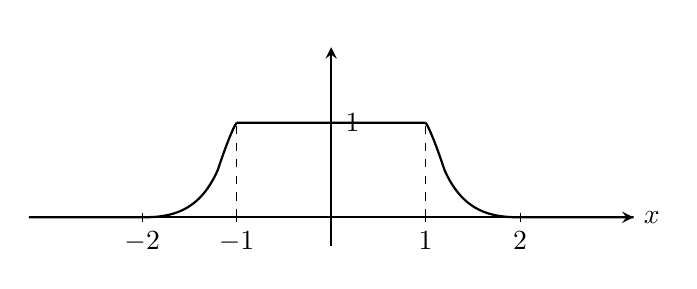
\begin{tikzpicture}[scale=1.2]

  % Axes
  \draw[thick, ->, >=stealth] (-3.2, 0) -- (3.2, 0) node[right] {$x$};
  \draw[thick, ->, >=stealth] (0, -0.3) -- (0, 1.8) node[above] {};

  % Courbe C^infty (fonction plateau)
  \draw[thick] 
    (-3.2, 0) -- (-2, 0)
    (-2, 0) .. controls (-1.7, 0) and (-1.4, 0.05) .. (-1.2, 0.5)
    (-1.2, 0.5) .. controls (-1.05, 0.95) and (-1.0, 1) .. (-1, 1)
    (-1, 1) -- (1, 1)
    (1, 1) .. controls (1.0, 1) and (1.05, 0.95) .. (1.2, 0.5)
    (1.2, 0.5) .. controls (1.4, 0.05) and (1.7, 0) .. (2, 0)
    (2, 0) -- (3.2, 0);

  % Tirets verticaux sur l'axe y
  \draw (0, 1) -- (0.05, 1) node[right] {$1$};

  % Marques sur l'axe x
  \foreach \x/\label in {-2/-2, -1/-1, 1/1, 2/2} {
    \draw (\x, 0.05) -- (\x, -0.05) node[below] {$\label$};
  }

  % Pointillés verticaux en x=-1 et x=1
  \draw[dashed] (-1, 0) -- (-1, 1);
  \draw[dashed] (1, 0) -- (1, 1);

\end{tikzpicture}
        \end{center}
        \[u_n(x)=\left(\frac{\chi}{n}\right)u(x)\]
        \begin{enumerate}
            \item $u_n\toninfty u$ dans $L^2(\R^d)$ TCD car $u_n(x)\toninfty$ pp et $|u_n|\le u$
            \item (lemme) $u_n\in H^1(\R^d)$ et
            \[\partial_j u_n(x)=\underset{=v_n}{\frac{1}{n}\partial_j \chi\left(\frac{x}{n}\right)u(x)}+\chi\left(\frac{x}{n}\right)\partial_j u(x)\]
            \begin{align*}
                \norme{v_n}^2_{L^2(\R^d)}&=\int_{\R^d} \frac{1}{n^2}|\partial_j \chi\left(\frac{x}{n}\right)|^2 |u(x)|^2\, dx\\
                &\le \frac{1}{n^2}\norme{\partial_j \chi}^2_{L^\infty(\R^d)}\norme{u}^2_{L^2(\R^d)}\toninfty 0
            \end{align*}
            Donc $\partial_j u_n\to \partial_j u$ dans $L^2(\R^d)$. On a donc prouvé que $u_n\to u$ dans $H^1(\R^d)$.\\
            2ème étape: Régularisation\\
            $\rho\in\Dr(\R^d),\rho\ge 0,\int_{\R^d}\rho=1,\rho_n(x)=n^d\rho(nx),\int\rho_n=1$.\\
            Soit $v\in H^1_c(\R^d)$. $v_n=\rho*v$ à support compact car $\rho_n$ et $v$ le sont et $C^\infty$ car $\rho_n$ est $C^\infty$.
            \begin{align*}
                \norme{v_n-v}_{L^2(\R^d)}&=\norme{\hat{v_n}-\hat{v}}_{L^2(\R^d)}\\
                &=\norme{(\hat{\rho_n}-1)\hat{v}}_{ L^2(\R^d)}\\
                &\le \norme{\hat{\rho_n-1}}_{L^\infty(\R^d)} \norme{\hat{v}}_{L^2}
            \end{align*}
            \begin{align*}
                \widehat{\varphi_n}(\xi)&=\int_{\R^d} e^{-2 i\pi x\xi}\rho(nx)n^d\, dx\\
                &=\int_{\R^d}e^{-2i\pi \frac{y}{n}\xi}\rho(y)\, dy\\
                &=\widehat{\rho}\left(\frac{\xi}{n}\right)\toninfty \widehat{\rho}(0)\qquad \text{ uniformément en $\xi$}
            \end{align*}
            Car $\widehat{\rho}\in \Sr(\R^d)$ car $\rho\in \Dr(\R^d)\subset \Sr(\R^d)$. $\widehat{\rho}(0)=\int \rho=1$, donc $\widehat{\rho_n}-1\toninfty 0$ uniformément.
            \[\norme{\widehat{\rho_n}-1}_{L^\infty(\R^d)}\toninfty 0\]
            Donc $\norme{v_n-v}_{L^2}\toninfty 0$. $\partial_j v_n=\rho_n*\partial_j v$, et on fait la même chose.
            \[\norme{\partial_j v_n -\partial_j v}_{L^2(\R^d)}\toninfty 0\]
            \item Conclusion: Soit $u\in H^1(\R^d),\epsilon>0$,
            \begin{enumerate}
                \item $\exists v\in H_C^1(\R^d),\norme{u-v}_{H^1}(\R^d)<\frac{\epsilon}{2}$
                \item $\exists w\in \Dr(\R^d),\norme{w-v}_{H^1(\R^d)}<\frac{\epsilon}{2}$,
                \[\norme{u-w}_{H^1(\R^d)}\le \frac{\epsilon}{2}+ \frac{\epsilon}{2}=\epsilon\]
            \end{enumerate}
        \end{enumerate}
    \end{proof}

    \begin{tm}{}{}
        Soit $s\in \N$,
        \[H^s(\R^d)=\{u\in L^2(\R^d),\int_{\R^d}(1+|\xi|^2)^s|\hat{u}(\xi)|^2\, d\xi <+\infty\}\]
        De plus, $N_s(u)=\left(\int_{\R^d} (1+|\xi|^2)^s|\hat{u}(\xi)|^2\, d\xi \right)^{\frac{1}{2}}$ est une norme sur $H^s(\R^d)$ équivalente à la norme $H^s$
    \end{tm}

    \begin{proof}
        Cas $s=1$, $u\in H^1(\R^d)$, alors $u\in L^2(\R^d)$ donc $\widehat{u}\in L^2(\R^d)$.\\
        Rappel: $\forall u\in \Dr(\R^d)$, $\widehat{\partial_j u}(\xi)=2i \pi \xi_j \widehat{u}(\xi)$. $\exists (u_n)_n$ une suite de $\Dr(\R^d)$ telle que
        \[\norme{u-u_n}_{H^1(\R^d)}\toninfty 0\]
        De plus, $\widehat{\partial_j u_n}(\xi)=2i\pi \xi_j \widehat{u_n}(\xi)$
        \begin{align*}
            \forall \varphi\in \Dr(\R^d),\quad \int_{\R^d}\widehat{\partial_j u_n}\varphi&=2i\pi \int_{\R^d} \xi_j \widehat{u_n}(\xi)\varphi(\xi)\, d\xi\toninfty 2i\pi \int_{\R^d}\xi_j \widehat{u}(\xi)\varphi(\xi)\, d\xi\\
            \int_{\R^d}\partial_j u_n\widehat{\varphi} &=\\
            \int_{\R^d}\widehat{\partial_j u}\varphi=\int_{\R^d}\partial_j u\widehat{\varphi}\underset{n\to \infty}{\longleftarrow}&
        \end{align*}
        Donc $\widehat{\partial_j}u=2i\pi \xi_j \widehat{u}(\xi)$ donc $\int 4\pi \xi_j^2 |\widehat{u}(\xi)|\, d\xi<+\infty$. Ainsi, $\int(1+|\xi|^2)|\widehat{u}(\xi)|^2\, d\xi<+\infty$.\\
        Réciproque: On suppose $u\in L^2(\R^d)$ et $(1+|\xi|^2)^{\frac{1}{2}}\widehat{u}(\xi)\in L^2(\R^d)$.\\
        En particulier, $2i\pi \xi_j \widehat{u}(\xi)$ est dans $L^2$, $v_j=\Fr^{-1}(2i\pi \xi_j \widehat{u}(\xi))\in L^2(\R^d)$,
        \begin{align*}
            \forall \varphi\in \Dr(\R^d),\quad \sca{\partial_j u,\varphi}&=-\sca{u,\partial_j \varphi}\\
            &=-\int_{\R^d}u\partial_j \varphi\\
            &=-\int_{\R^d}\widehat{u}\widehat{\partial_j \varphi}\\
            &=-\int_{\R^d}\widehat{u}(\xi)2i\pi \xi_j \widehat{\varphi}(\xi)\, d\xi\\
            &=\int_{\R^d}\underset{v_j}{\Fr^{-1}(2i\pi \xi_j \widehat{u}(\xi))}\varphi
        \end{align*}
        Donc $\partial_j u=v_j\in L^2(\R^d)$ et ceci $\forall j\in \{1,\ldots,d\}$, donc $u\in H^1(\R^d)$.\\
        Equivalence des normes: Il suffit de le démontrer pour $u\in \Dr(\R^d)$. Pour un tel $u$, $\widehat{\partial_j u}(\xi)=2i\pi \xi_j \widehat{u}(\xi)$, donc
        \begin{align*}
            \norme{u}_{H}^2=\int_{\R^d}|u|^2+\int_{\R^d}|\nabla u|^2&=\int_{\R^d}|\widehat{u}|^2+\int_{\R^d}4\pi^2|\xi|^2 |\widehat{u}(\xi)|^2\, d\xi\\
            &\le 4\pi^2N_1(u)^2\ge N_1(u)^2
        \end{align*}
    \end{proof}

    \begin{ra}{}{}
        \[C_0(\R^d)=\{\funto{u}{\R^d}{\R}\text{ continue, }\lim_{|x|\to\infty}u(x)=0\}\]
    \end{ra}

    \begin{tm}{Injections de Sobolev}{}
        Pour $d\in \N^*,s\in \N$
        \begin{enumerate}
            \item Si $s>\frac{d}{2}$, alors $H^s(\R^d)\subset C_0(\R^d)$ avec injection continue:
            \[\exists c>0,\forall u\in H^s(\R^d),\norme{u}_{C_0(\R^d)}\le c\norme{u}_{H^s(\R^d)}\]
            \item Si $s<\frac{d}{2}$, alors $H^s(\R^d)\subset L^{p^*}(\R^d)$ avec $p^*=\frac{2d}{d-2s}$, avec injection continue:
            \[\exists c>0,\forall u\in  H^s(\R^d),\norme{u}_{L^{p^*}}(\R^d)\le c\norme{D^s u}_{L^s(\R^d)}\]
            \item Si $s=\frac{d}{2}$, alors $\forall p\in [2,+\infty[,H^s(\R^d)\subset L^p(\R^d)$ avec injection continue:
            \[\exists c_p>0,\forall u\in H^s(\R^d),\norme{u}_{L^p(\R^d)}\le c_p\norme{u}_{H^s(\R^d)}\]
        \end{enumerate}
    \end{tm}

    \begin{re}{}{}
        Pour $s<\frac{d}{2},p^*>2$, par Hölder, $u\in L^p(\R^d),\forall p\in [2,p*]$
    \end{re}

    \begin{re}{}{}
        La valeur de $p^*$ peut se déterminer par changement d'échelles:\\
        Si $\exists p^*\in [2,+\infty[$, tel que $\norme{u}_{L^{p^*}}\le c\norme{D^s u}_{L^2}$ alors nécessairement $p^*=\frac{2d}{d-2s}$
    \end{re}

    \begin{proof}
        On applique l'inégalité à $u_\lambda(x)=u(\lambda x),\lambda\in \R^{+*}$.
        \begin{align*}
            \norme{u_\lambda}_{L^{p^*}}&=\left(\int_{\R^d}|u(\lambda x)|^{p^*}\, dx\right)^{\frac{1}{p^*}}\\
            &=\left(\int_{\R^d}|u(y)|^{p^*\lambda^{-d}}\, dy\right)^{\frac{1}{p^*}}\\
            &=\lambda^{\frac{-d}{p^*}}\norme{u}_{L^{p^*}}
        \end{align*}
        \[D^s u_\lambda=\lambda^s( D^s u)(\lambda x)\]
        \[\norme{D^s u_\lambda}_{L^2}=\lambda^s\left(\int_{\R^d}\left| D^s u(\lambda x)\right|^2\right)^{\frac{1}{2}}\]
        Même calcul $y=\lambda x$
        \[\norme{D^s u_\lambda}_{L^2}=\lambda^s\lambda^{-\frac{d}{2}}\norme{D^s u}_{L^2}\]
        \begin{align*}
            \lambda^{-\frac{d}{p^*}}\norme{u}_{L^p}&\le C\lambda^{s-\frac{d}{2}}\norme{D^s u}_{L^2}\\
            \norme{u}_{L^{p^*}}&\le C\lambda^{\frac{d}{p^*}+s-\frac{d}{2}}\norme{D^s u}_{L^2}
        \end{align*}
        Donc $\frac{d}{p^*}+s-\frac{d}{2}=0\implies p^*=\frac{2d}{d-2s}$
    \end{proof}

    \begin{lm}{}{}
        Si $\funto{u}{\R^d}{\R}$ mesurable, $p\in [1,+\infty[$, alors
        \[\int_{\R^d}|u(x)|^p\, dx=\int_{0}^{+\infty}p\lambda^{p-1}\left|\{|u|>\lambda\}\right|\, d\lambda\]
    \end{lm}

    \begin{proof}
        \begin{align*}
            \int_{0}^{+\infty}p\lambda^{p-1}|\{|u|>\lambda\}|\, d\lambda&=\int_{0}^{+\infty}p\lambda^{p-1}\left(\int_{\R^d} \1_{|u|>\lambda}(x)\, dx\right)\, d\lambda\\
            &=\int_{\R^d}\left(\int_{0}^{+\infty}p\lambda^{p-1}\1_{|u(x)|>\lambda}\, d\lambda \right)\, dx\\
            &=\int_{\R^d}\int_{0}^{+\infty}p\lambda^{p-1}\, d\lambda\\
            &=\int_{\R^d}|u(x)|^p\, dx
        \end{align*}
    \end{proof}

    \begin{proof}
        Preuve du théorème: \begin{enumerate}
            \item $s>\frac{1}{2}$,
            \begin{align*}
                \int_{\R^d}|\hat{u}(\xi)|\, d\xi&=\int_{\R^d}(1+|\xi|^2)^{\frac{s}{2}}|\hat{u}(\xi)|\frac{1}{(1+|\xi|^2)^{\frac{s}{2}}}\, d\xi\\
                &\overset{\text{Cauchy-Schwarz}}{\le}\underset{N_s(u)\le c\norme{u}_{H^s(\R^d)}}{\left(\int_{\R^d}(1+|\xi|^2)^s|\hat{u}(\xi)|^2\, d\xi\right)^{\frac{1}{2}}}\left(\int_{\R^d}\frac{d\xi}{(1+|\xi|^2)^s}\right)^{\frac{1}{2}}
            \end{align*}
            $\int_{\R^d}\frac{d\xi}{(1+|\xi|^2)^s}=\int_{0}^{+\infty}\frac{C_d r^{d-1}\, dr}{(1+r^2)^s}$ et $\frac{r^{d-1}}{(1+r^2)^s}\underset{r\to \infty}{\sim}\frac{1}{r^{2s-d+1}}$ et on a que $2s-d+1>1$ donc
            \[\int_{\R^d}\frac{d\xi}{(1+|\xi|^2)^s}<+\infty\]
            Donc $\hat{u}\in L^1(\R^d)$, d'où $u$ continue, et par Riemann-Lebesgue $\lim_{|x|\to \infty}u(x)=0$, de plus
            \begin{align*}
                \norme{u}_{C_0(\R^d)}=\sup_{x\in \R^d}|u(x)|&\le \norme{\hat{u}}_{L^1(\R^d)}\\
                &\le C_{d,s}\norme{u}_{H^s(\R^d)}
            \end{align*}
            \item Idée: On pose $A>0$ et $u_+=\Fr^{-1}(\hat{u}(\xi)\1_{|\xi|>A}),u_-==\Fr^{-1}(\hat{u}(\xi)\1_{|\xi|<A})$, on a $u_+ +u_-=u$. On pose $\lambda >0$, on a
            \[\{|u|>\lambda\}\subset \{|u_+|>\frac{\lambda}{2}\}\cup \{|u_-|>\frac{\lambda}{2}\}\]
            Donc
            \[|\{|u|>\lambda\}|\le \left|\{|u_+|>\frac{\lambda}{2}\}\right|+ \left|\{|u_-|>\frac{\lambda}{2}\}\right|\]
            \begin{align*}
                \norme{u_-}_{L^\infty}&\le \norme{\hat{u_-}}_{L^1}=\int_{\R^d}|\hat{u_-}(\xi)|\, d\xi=\int_{|\xi|<A}|\hat{u}(\xi)|\, d\xi\\
                &\le \int_{|\xi|<A}|\xi|^s|\hat{u}(\xi)|\xi|^{-s}\, d\xi\\
                &\overset{\text{C-S}}{\le}\underset{\le N_s(u)\le c\norme{u}_{H^s(\R^d)}}{\left(\int_{|\xi|<A}|\xi|^{2s}|\hat{u}(\xi)|^2\, d\xi\right)^{\frac{1}{2}}} \left(\int_{|\xi|<A}\frac{d\xi}{|\xi|^{2s}}\right)^{\frac{1}{2}}
            \end{align*}
            \[\int_{|\xi|<A}\frac{d\xi}{|\xi|^{2s}}=c_d\int_{0}^{A}\frac{r^{d-1}\, dr}{r^{2s}}=c_d\int_{0}^{A}r^{d-2s-1}\, dr=c_d\frac{A^{d-2s}}{d-2s}\qquad \text{ car $d-2s>0$}\]
            Donc
            \[\norme{u_-}_{L^\infty}\le C\norme{u}_{H^s(\R^d)}A^{\frac{d}{2}-s}\]
            où la constante $C$ est indépendante de $A$ et de $u$. On choisit $A=A(\lambda)$ tel que
            \[C\norme{u}_{H^s(\R^d)}A(\lambda)^{\frac{d}{2}-s}=\frac{\lambda}{2}\quad\text{i.e.}\quad A(\lambda)=\left(\frac{\lambda}{2C\norme{u}_{H^s(\R^d)}}\right)^{\!\frac{1}{\frac{d}{2}-s}}\]
            Alors $\norme{u_-}_{L^\infty}\le\frac{\lambda}{2}$, donc $\left\{|u_-|>\frac{\lambda}{2}\right\}=\emptyset$ et $\left|\left\{|u_-|>\frac{\lambda}{2}\right\}\right|=0$.\\
            Reste à majorer $\left|\left\{|u_+|>\frac{\lambda}{2}\right\}\right|$. Par l'inégalité de Markov:
            \[\left|\left\{|u_+|>\frac{\lambda}{2}\right\}\right|\le\frac{4}{\lambda^2}\norme{u_+}_{L^2}^2=\frac{4}{\lambda^2}\int_{|\xi|>A(\lambda)}|\hat{u}(\xi)|^2\, d\xi\]
            Par le lemme de layer-cake et en échangeant les intégrales (Fubini, les intégrandes étant positifs):
            \begin{align*}
                \norme{u}_{L^{p^*}}^{p^*}&=\int_{0}^{+\infty}p^*\lambda^{p^*-1}|\{|u|>\lambda\}|\, d\lambda\\
                &\le \int_{0}^{+\infty}4p^*\lambda^{p^*-3}\left(\int_{|\xi|>A(\lambda)}|\hat{u}(\xi)|^2\, d\xi\right)d\lambda\\
                &=\int_{\R^d}4p^*|\hat{u}(\xi)|^2\left(\int_{0}^{C|\xi|^{\frac{d}{2}-s}\norme{u}_{H^s}}\lambda^{p^*-3}\, d\lambda\right)d\xi\\
                &=\int_{\R^d}\frac{4p^*}{p^*-2}|\hat{u}(\xi)|^2\left(C|\xi|^{\frac{d}{2}-s}\norme{u}_{H^s}\right)^{p^*-2}d\xi\\
                &=C\norme{u}_{H^s}^{p^*-2}\int_{\R^d}|\xi|^{\frac{d}{p^*}(p^*-2)}|\hat{u}(\xi)|^2\, d\xi
            \end{align*}
            Or $\dfrac{d}{p^*}(p^*-2)=d\!\left(1-\dfrac{2}{p^*}\right)=d\!\left(1-\dfrac{d-2s}{d}\right)=2s$.
            Donc:
            \[\norme{u}_{L^{p^*}}^{p^*}\le C\norme{u}_{H^s}^{p^*-2}\int_{\R^d}|\xi|^{2s}|\hat{u}(\xi)|^2\, d\xi\le C\norme{u}_{H^s}^{p^*-2}\cdot N_s(u)^2\le C\norme{u}_{H^s}^{p^*}\]
            Ainsi $\norme{u}_{L^{p^*}}\le C\norme{u}_{H^s(\R^d)}$.
            \item $s=\frac{d}{2}$, $p\in[2,+\infty[$. On pose
            \[\tilde{s}=\frac{d}{2}\!\left(1-\frac{2}{p}\right)<\frac{d}{2}=s\]
            (et $\tilde{s}\ge 0$ car $p\ge 2$, avec $\tilde{s}>0$ car $p<+\infty$). Puisque $\tilde{s}<s$, on a $(1+|\xi|^2)^{\tilde{s}}\le (1+|\xi|^2)^s$, donc
            \[\int_{\R^d}(1+|\xi|^2)^{\tilde{s}}|\hat{u}(\xi)|^2\, d\xi\le\int_{\R^d}(1+|\xi|^2)^s|\hat{u}(\xi)|^2\, d\xi<+\infty\]
            En particulier $\norme{u}_{H^{\tilde{s}}(\R^d)}\le C_s\norme{u}_{H^s(\R^d)}$. Comme $\tilde{s}<\frac{d}{2}$, on peut appliquer le cas (2) à l'exposant $\tilde{s}$:
            \[\norme{u}_{L^{p^*(\tilde{s})}}\le C\norme{u}_{H^{\tilde{s}}}\le C'\norme{u}_{H^s}\]
            où $p^*(\tilde{s})=\dfrac{2d}{d-2\tilde{s}}$. On calcule:
            \[p^*(\tilde{s})=\frac{2d}{d-2\cdot\frac{d}{2}\!\left(1-\frac{2}{p}\right)}=\frac{2d}{d-d\!\left(1-\frac{2}{p}\right)}=\frac{2d}{\frac{2d}{p}}=p\]
            Donc $\norme{u}_{L^p}\le C'\norme{u}_{H^s(\R^d)}$, ce qui conclut la démonstration.
        \end{enumerate}
    \end{proof}

    (Voir avec Nicolas et William)

    \begin{tm}{Inégalité de Poincaré-Wirtinger}{}
        Soit $\Omega$ un ouvert borné de classe $C^1$. Alors il existe $C>0,$
        \[\forall u\in H^1(\Omega),\int_{\Omega}(u-\dashint_{\Omega} u)^2\le C\int_{\Omega}|\nabla u|^2\]
    \end{tm}

    \begin{proof}
        Par l'absurde, s'il n'exite par une telle constante, alors $\exists (u_n)_\nN,u_n\in H'(\Omega),$
        \[\int_{\Omega} |\nabla u|^2 \toninfty 0\qquad \int_{\Omega}(u_n-\dashint_{\Omega} u_n)^2=1\]
        Soit $\nu_n= u_n-\dashint_\Omega u_n$. On a 
        \[\cho{\int_\Omega |\nabla \nu_n|^2\toninfty 0\\ \int_\Omega \nu_n^2=1 \\\int_\Omega \nu_n =0}\]
        Extraction: Soit $(\nu_{\theta(n)})_\nN$ vérifie
        \[\cho{\nabla \nu_{\theta(n)}\to \nabla \nu\text{ dans $L^2(\Omega)$}\\ \nu_{\theta(n)}\text{ dans $L^2(\Omega)$}}\]
        \[0=\int_\Omega \nu_{\theta(n)}\toninfty \int_{\Omega}\nu\]
        \[1=\int_\Omega \nu_{\theta(n)}^2\toninfty \int_\Omega \nu^2\]
        Soit $l\in \Dr(\Omega)$,
        \[\int_\Omega \nabla \nu_{\theta(n)}l\toninfty\int_\Omega\nabla \nu l\text{ (cv faible $L^2$)}\]
        \[\left|\int_\Omega \nabla \nu_{\theta(n)}l\right|\le \norme{\nabla \nu_{\theta(n)}}_{L^2(\Omega)}\norme{l}_{L^2(\Omega)}\toninfty 0\]
        Donc $\nabla v=0$, donc $\nu$ constante $\int v=0$, donc $\nu=0$. Mais $\int_{\Omega}\nu^2=1$. Contradiction
    \end{proof}

    \begin{df}{}{}
        Soit $\Omega$ un ouvert de $\R^d$. On définit $H_0^1(\Omega)$ comme l'adhérence dans $H^1(\Omega)$ de l'espace $\Dr(\Omega)$.
    \end{df}

    \begin{re}{}{}
        $H_0^1(\R^d)=H^1(\R^d)$. Mais si $\Omega\subsetneq \R^d$, alors $H_0^1(\R^d)\subsetneq H^1(\Omega)$\\
    \end{re}

    \begin{prop}{}{}
        Soit $\Omega$ ouvert borné de classe $C^1$, et $u\in H^1(\Omega)\cap C^0(\overline{\Omega})$, alors
        \[u\in H_0^1(\Omega)\iff u_{|\partial \Omega}=0\]
    \end{prop}

    \begin{proof}
        cf Brèzis théorème 9.17
    \end{proof}

    \begin{tm}{Inégalité de poincaré}{}
        Soit $\Omega$ un ouvert borné de classe $C^1$. Alors $\exists c>0$ telle que $\forall u\in H_0^1(\Omega)$, 
        \[\int_{\Omega}u^2\le c\int_{\Omega}|\nabla u|^2\]
    \end{tm}

    \begin{proof}
        Par densité, il suffit de le démontrer pour $u\in \Dr(\Omega), \Omega\subset [0,R]^d,R>0$. On étend $u$ par $u(x)=0,\forall x\notin \Omega$,
        \[u(x)^2=\int_{-R}^{x_d}\partial_d (u(x_1,\ldots,x_{d-1},t))^2\, dt=2\int_{-R}^{x_d}u(x',t)\partial_d u(x',t)\, dt\]
        \begin{align*}
            u(x)^2&\le 2\int_{-R}^{x_d} |u(x',t)||\partial_d u(x',t)|\, dt\\
            \int_\Omega u(x)^2\, dx &\le 2\int_\Omega\int_{-R}^{R}|u(x',t)||\nabla u(x',t)|\, dt\, dx\\
            \int_\Omega u^2&\le 2\int_{[-R,R]^d}\int_{-R}^{R}|u(x',t)||\nabla u(x',t)|\, dt\, dx'\, dx_d\\
            &=4R \int_{[-R,R]^{d-1}}\int_{-R}^{R}|u(x',t)||\nabla u(x',t)|\, dt\, dx'\\
            &=4R \int_{[-R,R]^d}|u(x)||\nabla u(x)|\, dx=4R\int_{\Omega}|u||\nabla u|\\
            &\le 4R \left( \int_{\Omega}|u|^2\right)^{\frac{1}{2}} \left(\int_{\Omega}|\nabla u|^2\right)^{\frac{1}{2}}
        \end{align*}
    \end{proof}
    
    \begin{cor}{}{}
        Dans $H_0^1(\Omega)$, le produit scalaire $(u|v)_{H_0^1}=\int_\Omega \nabla u\cdot \nabla v$ est équivalent au produit scalaire $H^1$.
    \end{cor}

    \begin{proof}
        $\forall u\in H_0^1(\Omega)$
        \begin{align*}
            \norme{u}^2_{H^1(\Omega)}&=\int_\Omega u^2+\int_\Omega |\nabla u|^2\le (1+c)\int_\Omega |\nabla u|^2\\
            &\ge \int_\Omega |\nabla u|^2=\norme{u}^2_{H_0^1(\Omega)}
        \end{align*}
    \end{proof}

    \chapter{Equations aux dérivées partielles elliptiques}

    \section{Equation de Poisson}

    Soit $\Omega$ ouvert borné de $\R^d$ (de classe $C^1$). On s'intéresse au problème
    \[\cho{-\Delta u=f\text{ dans $\Omega$}\\u_{|\partial\Omega}=0}\quad(*)\]
    $f$ est une donnée, $u$ inconnue.
    \begin{center}
        Question: Existence ? Unicité ? Si existence et unicité $f\mapsto u$ continue ?\\
    \end{center}

    \begin{df}{}{}
        On définie $H^{-1}(\Omega)=\left(H_0^1(\Omega)\right)'\supset L^2(\Omega)$
    \end{df}

    \begin{df}{}{}
        Soit $f\in H^{-1}(\Omega)$, on appelle solution faible de $(*)$ un $u\in H_0^1(\Omega)$ telle que
        \[\forall v\in H_0^1(\Omega),\int_\Omega \nabla u\nabla v=\sca{f,v}\]
        Formellement, ceci équivaut à $\sca{-\Delta u,v}=\sca{f,v}$:
        \begin{itemize}
            \item $u\in H_0^1(\Omega)$ traduit le fait que $u_{|\partial \Omega}=0$ pour $u\in H^1(\Omega)$.
            \item $\int_\Omega \nabla u\nabla v=\sca{f,v}$ implique $-\Delta u=f$ au sens des distributions
            \item Si $u\in C^2(\Omega)\cap C^0(\overline{\Omega})$ et $f\in C^0(\overline{\Omega}), u_{|\partial \Omega}=0$ et si $\Delta u=f$, alors
            \[\forall v\in \Dr(\Omega),\int_\Omega (-\Delta u) v=\int_\Omega fv\]
            Ceci $\forall v\in \Dr(\Omega)$ donc $\forall v\in H_0^1(\Omega)$
            \item Si $u$ est solution faible et qu'on sait que $u\in C^2(\Omega)\cap C^0(\overline{\Omega})$, alors:
            \[\forall v\in \Dr(\Omega),\int_\Omega \nabla u\nabla v=\sca{f,v}\]
            \[\int_\Omega (-\Delta u)v=\sca{f,v}\]
            En particulier, $\forall v\in \Dr(\Omega)$,
            \[\left|\sca{f,v}\right|\le \norme{-\Delta u}_{L^2(\Omega)}\norme{v}_{L^2(\Omega)}\] 
            donc $f\in L^2(\Omega)$ au sens où
            \[\exists! \tilde{f}\in L^2(\Omega),\sca{f,v}=\int_\Omega \tilde{f}v,\forall v\in \Dr(\Omega) \text{ donc $\forall v\in H^1(\Omega)$}\]
            On confond $f$ et $\tilde{f}$. Ainsi, $\forall v\in \Dr(\Omega),$
            \begin{align*}
                \int_\Omega (-\Delta u)v&=\int_\Omega fv\\
                \int_\Omega (-\Delta u-f)v&=0
            \end{align*}
            D'où $-\Delta u -f=0$ et donc $-\Delta u=f$
        \end{itemize}
    \end{df}

    \begin{tm}{}{}
        Soit $\Omega$ un ouvert borné de classe $C^1$. Soit $f\in H^{-1}(\Omega)$.\\
        Alors $\exists! u\in H_0^1(\Omega)$ solution faible de $(*)$
    \end{tm}

    \begin{proof}
        On sait que $(u,v)_{H_0^1}=\int_\Omega \nabla u\nabla v$ est un produit scalaire sur $H_0^1(\Omega)$ équivalent au produit scalaire sur $H^1$.\\
        D'autre part, $H_0^1$ est un \sev fermé de $H^1$, donc un espace de Hilbert (Pour le produit scalaire $H^1$). C'est donc aussi un Hilbert pour $(\cdot,\cdot)_{H_0^1}$.\\
        Par le théorème de représentation de Riesz:
        \[\forall T\in (H_0^1(\Omega))',\exists! u\in H_0^1(\Omega),\forall v\in H_0^1(\Omega),(u,v)_{H_0^1(\Omega)}=T(v)\]
        On applique ça à $T=f$ et on obtient le résultat
    \end{proof}

    \begin{prop}{}{}
        La solution définie ci-dessus vérifie
        \[\norme{u}_{H_0^1(\Omega)}\le \norme{f}_{H^{-1}(\Omega)}\]
        Autrement dit, l'application $f\mapsto u$ est linéaire, continue et de norme au plus 1.
    \end{prop}

    (Voir cours Nicolas, p.29)

    \[(**)\qquad\cho{-\text{div}(A\nabla u)=f\text{ dans $\Omega$}\\ u_{|\partial \Omega}=0}\]
    $\funto{A}{\Omega}{\R^{d\times d}}$, $A$ est bornée $(L^\infty)$, $A$ est uniformément elliptique:
    \[\exists \alpha>0,\forall \xi\in \R^d,\xi^{T}A(x)\xi\ge \alpha |\xi|^2\]

    \begin{re}{}{}
        Une autre façon d'écrire l'équation est:
        \[-\sum_{j=1}^d\sum_{i=1}^{d}\partial_i (a_{ij}(x)\partial_j u(x))=f(x)\]
        Si $A$ est $C^1$, ceci s'écrit aussi
        \begin{align*}
            -\sum_j\sum_i a_{ij} \partial_{ij} u - \sum_j \sum_i \partial_i a_{ij}\partial_{j}u&=f\\
            -\text{Tr} (AD^2u) -\text{div}(A)\cdot \nabla u&= f
        \end{align*}
        Si $A=\Id$, on retrouve $-\Delta u =f$
    \end{re}

    \begin{df}{}{}
        On appelle solution faible de $(**)$ toute fonction $u\in H_0^1(\Omega)$ telle que $\forall v\in H_0^1(\Omega)$,
        \[\int_{\Omega} \nabla v^T A\nabla u=\sca{f,v}\]
    \end{df}
    
    \begin{tm}{}{}
        Soit $\Omega$ ouvert borné de classe $C^1$ de $\R^d$. Soit $f\in H{-1}(\Omega)$. Soit $A\in L^\infty(\Omega,\R^{d\times d})$ uniformément elliptique. Alors $\exists! u \in H_0^1(\Omega)$ solution faible de $(**)$.\\
        De plus, l'application $\fundf{H^{-1}(\Omega)}{H_0^1(\Omega)}{f}{u}$ solution faible de $(**)$ est linéaire continue.
    \end{tm}

    \begin{proof}
        On applique Lax-Milgram avec $V=H_0^1(\Omega)$
        \[a(u,v)=\int_\Omega \nabla v^T A\nabla u, b(v)=\sca{f,v}\]
        \begin{itemize}
            \item $b$ continue: $|b(v)|=|\sca{f,v}|\le \norme{f}_{H^{-1}} \norme{v}_{H_0^1}$
            \item $a$ continue
            \begin{align*}
                a(u,v)&=\sum_{i=1}^{d}\sum_{j=1}^{d} \int_{\Omega} a_{ij}\partial_i v\partial_j u \qquad \text{ Pour $\beta=\sup \norme{a_{ij}}_{L^\infty}<+\infty$}\\
                |a(u,v)|&\le \sum_i \sum_j \int_\Omega |a_{ij}||\partial_i v||\partial_j u|\\
                &\le \beta \int_{\Omega} \left(\sum_i |\partial_i v|\right)\left(\sum_j |\partial_j u|\right)\\
                &\le \beta d \int_\Omega |\nabla u||\nabla v|\le \beta d \norme{\nabla u}_{L^2} \norme{\nabla v}_{L^2}
            \end{align*}
            \item $a$ est coercive
            \[a(u,u)=\int_\Omega\nabla u^T A\nabla u \ge \int_{\Omega} \alpha |\nabla u|^2=\alpha \norme{u}_{H_0^1}^2\]
        \end{itemize}
        Lax-Milgram: $\exists! u\in H_0^1(\Omega)$ solution de $\forall v\in H_0^1(\Omega),$
        \[a(u,v)=b(f)\]
        De plus, si on choisit $v=u$,
        \[\alpha \int_{\Omega}|\nabla u|^2\le \int_{\Omega}\nabla u^T A\nabla u=\sca{f,u}\le \norme{f}_{H^{-1}}\norme{u}_{H_0^1}\]
        \[\norme{u}_{H_0^1}\le \frac{\norme{f}_{H^{-1}}}{\alpha}\]
    \end{proof}

    \section{Analyse spectrale du laplacien}

    \begin{df}{}{}
        Soit $V$ un espace de Hilbert, soit $\funto{T}{V}{V}$ linéaire. On dit que $T$ est auto-adjoint si $\forall u\in V,\forall v\in V, (Tu|v)=(u|Tv)$
    \end{df}

    \begin{df}{}{}
        Soit $V$ un espace de Hilbert (Banach suffit). Soit $\funto{T}{V}{V}$ linéaire. On dit que $T$ est compacte si $\overline{T(B_1)}$ est compacte.
    \end{df}

    \begin{tm}{Théorème  spectral pour les opérateurs auto-adjoints compacts}{}
        Soit $V$ un espace de Hilbert séparable. Soit $\funto{T}{V}{V}$ linéaire, auto-adjointe, compacte.\\
        Alors $\exists(e_n)_{\nN}$ base hilbertienne de $V$ telle que $T e_n=\lambda_n e_n$, avec $\lambda_n\in R$ et $\lim_{\toninfty} \lambda_n=0$
    \end{tm}

    On applique ça à $(-\Delta)^{-1}$ dans $V=L^2(\Omega)$. On sait que $\forall f\in L^2(\Omega),\exists! u\in H_0^1(\Omega)$, solution faible de $-\Delta u=f$.\\
    On note $\fundfto{(-\Delta)^{-1}}{L^2(\Omega)}{H_0^1(\Omega)\subset L^2(\Omega)}{f}{u}$ solution faible.\\
    $(-\Delta)^{-1}$ est linéaire continue de $L^2$ dans $L^2$. De plus, $H_0^1(\Omega)\subset L^2(\Omega)$ est compact, donc $(\Delta)^{-1}$ est compacte.\\
    $(-\Delta)^{-1}$ auto-adjointe ?\\
    $f\in L^2(\Omega),g\in L^2(\Omega)$,
    \[\left((-\Delta)^{-1} f | g\right)_{L^2}=\int_\Omega ug\]
    Où $u$ vérifie que $\forall v\in H_0^1(\Omega),\int_\Omega \nabla u\nabla v=\int_\Omega fv$.\\
    Par ailleurs, $v=(-\Delta)^{-1}g$ vérifie
    \[\forall w\in H_0^1,\int_\Omega \nabla v\nabla w=\int_\Omega g w\]
    On choisit $w=u$ dans cette formulation.
    \[\left(f|(-\Delta)^{-1} g\right)=\int_\Omega fv =\int_\Omega\nabla v\nabla u=\int_\Omega gu=\left((-\Delta)^{-1} f|g\right)\]
    (Voir photos pour le reste 26/03)

    \begin{prop}{}{}
        Soit $\Omega$ ouvert borné de classe $C^1$. Soit $(e_n)_n$ une base hilbertienne de $L^2(\Omega)$ constituée de vecteurs propres de $-\Delta$ ($-\Delta e_n=\lambda_n e_n$) avec $\lambda_n >0$, $\lambda_n \toninfty +\infty$, alors
        \[\left(\frac{e_n}{\sqrt{\lambda_n}}\right)_\nN\]
        est une base hilbertienne de $H_0^1(\Omega)$
    \end{prop}

    \begin{ra}{}{}
        Le produit scalaire $H_0^1$ est
        \[\left(u|v\right)_{H_0^1}=\int_\Omega \nabla u\nabla v\qquad \text{(Equivalent au produit scalaire de $H^1$)}\]
    \end{ra}

    \begin{proof}
        $\forall \varphi\in H_0^1(\Omega)$,
        \[\int_\Omega\nabla e_n\cdot\nabla \varphi=\lambda_n \int_\Omega e_n\varphi,\forall n\in \N\]
        On choisit $\varphi=e_p,p\in \N,p\neq n$
        \begin{align*}
            \int_\Omega \nabla e_n\cdot\nabla e_p&=\lambda_n \int_\Omega e_n e_p=0\\
            \text{Pour $p=n$}\qquad \int_\Omega |\nabla e_n|^2&=\lambda_n\int_\Omega e_n^2=\lambda_n\\
            \int_\Omega \left|\nabla \left(\frac{e_n}{\sqrt{\lambda_n}}\right)\right|^2&=1
        \end{align*}
        Donc $\left(\frac{e_n}{\sqrt{\lambda_n}}\right)_\nN$ est orthonormée dans $H_0^1(\Omega)$.\\
        Reste à démontrer que $\text{Vect}\left(\frac{e_n}{\sqrt{\lambda_n}}\right)_\nN=V$ dense dans $H_0^1(\Omega)$.\\
        Autrement dit, $V^{\perp}=\{0\}$
        (Voir photos du 31/03 pour la suite de la preuve et pour la remarque) 
    \end{proof}

    \section{Principe du maximum}

    \begin{tm}{Principe du maximum faible}{}
        Soit $\Omega$ ouvert borné de classe $C^1$, $u\in C^1(\Omega)\cap C^0(\overline{\Omega})$.
        \begin{enumerate}
            \item Si $-Delta u\le 0$, alors $\max_\Omega u=\max_{\partial \Omega}u$
            \item Si $-\Delta u\ge 0$, alors $\min_\Omega u=\min_{\partial \Omega}u$
        \end{enumerate}
    \end{tm}

    \begin{re}{}{}
        Si $-\Delta u=0$, et $\Omega C^\infty$, alors $u$ est $C^\infty$. Donc elle  vérifie les hypothèses ci-dessus.
    \end{re}

    \begin{proof}
        \begin{enumerate}
            \item On commence par le cas où $-\nabla u<0$. Si $u$ atteint son maximum en $x_0\in \Omega$ (pas sur $\partial \Omega$), alors
            \[\nabla u(x_0)=0\text{ et } D^2u(x_0)\le 0\]
            (Voir photos pour suite de la démonstration 31/03)
        \end{enumerate}
    \end{proof}

    \begin{tm}{Principe du maximum fort}{}
        Soit $\Omega$ ouvert borné de classe $C^1$ et connexe, $u\in C^2(\Omega)\cap C^0(\overline{\Omega})$.
        \begin{enumerate}
            \item Si $-\Delta u\le 0$ et si $u$ atteint un maximum intérieur alors $u$ est constante.
            \item Si $-\Delta u\ge 0$ et si $u$ atteint un minimum intérieur alors $u$ est constante
        \end{enumerate}
    \end{tm}

    \begin{proof}
        Evans, Thm 4 paragraphe 6.4
    \end{proof}

    \begin{re}{}{}
        Ceci s'étend au cas où on remplace $-\nabla u$ par $-\text{div} (A\nabla u), A\in C^1(\Omega)$
    \end{re}

    \chapter{Equations parabolliques}

    \begin{center}
        On regarde l'équation:
    \end{center}

    \[\cho{\partial_t u-\text{div}(A\nabla u)=f\text{ dans $\R^+\times \Omega$}\\ u(0,x)= u_0(x)\text{ pp dans $\Omega$} \\ u_{|\partial \Omega}(t)=0 ,\forall t\in \R^+}\]
    
    \begin{center}
        Avec $A$ bornée, symétrique, et uniformément elliptique. Pour simplifier, on prend $A=\Id$
    \end{center}

    \begin{tm}{}{}
        Soit $\Omega$ ouvert borné de classe $C^1$. Soit $u_0\in L^2(\Omega)$.\\
        $\exists! u\in C^0(\R^+,L^2(\Omega))\cap C^1(\R^{+*},L^2(\Omega))\cap C^0(\R^{+*},H_0^1(\Omega))$ telle que
        \begin{itemize}
            \item $u(0,\cdot)=u_0$ pp dans $\Omega$
            \item $\forall t>0,\Delta u(t,\cdot)\in L^2(\Omega)$
            \item $\forall t>0,\partial_t u(t,\cdot)-\Delta u(t,\cdot)=0$
        \end{itemize}
    \end{tm}

    (Voir pour récup le cours du 07/04)
    
\end{document}